\documentclass{tufte-handout}
%\documentclass[a4paper, 12pt]{article}
\usepackage[utf8]{inputenc}

\usepackage{geometry}
\usepackage{graphicx}
\usepackage{xcolor}
\usepackage{verbatim}
\usepackage{xcolor}
\usepackage{amssymb}

\usepackage{caption}

\usepackage{indentfirst}
\usepackage{amsmath}
\usepackage{hyperref}
\usepackage{cleveref}
\usepackage[brazil]{babel}
\usepackage{minted}
\geometry{
  a4paper,
  total={170mm,350mm},
  left=10mm,
  top=5mm,
  bottom=30mm,
  textwidth=.60\paperwidth}

\iflarger
  \AtBeginDocument{%
  \fontsize{14}{16}\selectfont
  }
%\else
\fi


\definecolor{LightGray}{gray}{0.97}

\setminted[fortran]{  
    framesep=2mm,
    baselinestretch=1.2,
    bgcolor=LightGray,
    fontsize=\footnotesize,
    linenos,
} 

\graphicspath{ ./graficos/}

\hypersetup{
  pdfauthor={Jefter Santiago},
  pdftitle={Projeto 5 - Simulações de Monte Carlo},
  pdfcreator={Jefter Santiago}, 
  colorlinks=true,    % Color links instead of boxes
  linkcolor=blue,     % Color of internal links
  citecolor=green,    % Color of citation links
  urlcolor=blue,      % Color of URLs
}

% \usepackage{tgpagella}
% \usepackage{mathpazo} 

\title{Projeto 5 - Simulações de Monte Carlo}
\author{Jefter Santiago (12559016)}
\date{Entrega: 08/06/2024}

\begin{document}
\maketitle

\section{Introdução ao modelo de Ising}

Seja uma malha $2D$ com $L_x, L_y$ sítios nos eixos 
$x$ e $y$, respectivamente. Cada sítio tem um spin $\sigma_k = \{ -1, +1 \}$ associado. 

\begin{equation}
  \mathcal{H} = -\frac{J}{2} \sum_{i = 1}^{L_x}\sum_{\ell = 1}^{L_y} s(i, \ell) \left[s_{i-1,\ell}+s_{i+1, \ell}+s_{i, \ell-1}+s_{i, \ell + 1}\right]
  \label{eq:hamiltoniano_ising}
\end{equation}

trabalhamos apenas com malhas regulares quadradas, então $L \cdot L = N$, com $L=L_x=L_y$. 

a energia total é 

\begin{equation}
    E = \langle \mathcal{H} \rangle
\end{equation}


Buscamos entender a relação da energia, magnetização 
e a temperatura nesse sistema. 
Partindo da função de partição 

\begin{equation}
    \mathcal{Z}(\beta) = \sum_{i = 1}^{L} \sum_{\ell = 1}^{L} e^{-\beta E}
    \label{eq:funcao_particao}
\end{equation} 

onde $E$ é a energia dada pela (\ref{eq:hamiltoniano_ising}) e $\beta = 1/(K_bT)$.

Além disso, o calor específico pode ser obtido por 


\begin{equation}
    C = \frac{1}{N}\frac{\langle \mathcal{H}^2 \rangle - \langle \mathcal{H} \rangle^2}{k_B T^2}
    \label{eq:calor_especifico}
\end{equation}


Partindo do hamiltoniano (\ref{eq:hamiltoniano_ising}) e o spin $\sigma_k$ em cada sítio
$(i, \ell)$ podemos fazer diversas medidas como do sistema. 
Nesse trabalho estamos interessandos principalemente na energia média e magnetização média por sítio. 
Sendo a magnetização de um sítio sendo o estado do seu spin, dizemos que a magnetização 
total é simplesmente a soma de todos spins normalizada pela quantidade total de spins $N$.

\begin{equation}
    \langle m \rangle = \frac{1}{N} \sum_{i = 1}^{L} \sum_{\ell = 1}^{L} s(i,  \ell) 
    \label{eq:mag_media1}
\end{equation}

Da descrição da magnetização e a eq.(\ref{eq:mag_media1}) já podemos intuir que as configurações
correspondentes à máximo ou mínimo de magnetização são todos spins alinhados, sendo 
$\langle m \rangle_{\text{max}} = \pm 1$.

Queremos estudar a relação dessas medidas de energia e magnetização e suas relações com a 
temperatura. Por isso buscamos uma outra relação para a magnetização média por spin. Utilizando 
a função de partição(\ref{eq:funcao_particao}) para normalização dessa medida, temos $Z$ constante de normalização
e 

\begin{equation}
  \langle m \rangle =  \frac{1}{N} \frac{1}{Z} \left( \sum_{\sigma}^{N} e^{- \beta E} s_\sigma \right)
  \label{eq:mag_media_normalizada}
\end{equation}

\begin{equation}
  P(s) = \frac{e^{\beta s \Delta M}}{e^{-\beta s \Delta M} + e^{\beta s \Delta M}}
  \label{eq:prob_spin}
\end{equation}
\begin{equation}
  P(-s) = \frac{e^{-\beta s \Delta M}}{e^{-\beta s \Delta M} + e^{\beta s \Delta M}} 
 \label{eq:prob_spin_menos}
\end{equation}

onde $\Delta M$ é 

\begin{equation}
  \Delta M = J \left[ s(i-1, \ell) + s(i+1, \ell) + s(i, \ell -1) +  s(i, \ell+1) \right]
\end{equation}

Com essa descrição da magnetização média por spin podemos impor alguma dinâmica para o sistema e observar 
as medidas desejadas.
A dinâmica que trabalhamos nesse projeto que consiste em realizar alterar 
algum spin aleatório da malha de acordo com a probabilidade, isto é, sorteamos a chance de flipar o spin 
e se for menor ou maior (\ref{eq:prob_spin}) (\ref{eq:prob_spin_menos}) o estado é alterado e realizamos as medidas desejadas. 
Utilizamos simulação de Monte Carlo para realizar a dinâmica até que o sistema atinja um determinado equilíbrio. Nesse
método cada passo da simulação corresponde à dinâmica de alterar um spin para os $N$ spins do sistema. Tipicamente nas simulações
realizadas o número de passos de Monte Carlo utilizados foi $3000$, mas para observar alguns fenômenos foi necessário aumentar esse 
número. 


\section{Detalhes de implementação}

Todos os programas implementados no projeto seguem estruturas parecidas, portanto, foi
criado um módulo apenas com operações básicas envolvendo o modelo de Ising em $2$D. No arquivo
\verb|ising_modules.f| localizado na raiz do projeto estão as funções e rotinas gerais utilizadas
nas diferentes simulações.

Na descrição da malha 2D foram adotadas condições periódicas de contorno, então as bordas da grade 
estão conectadas e na discretização das posições dos spins foi utilizado um vetor de posição definido como 

\begin{minted}{fortran}
    dimension ipbc(0:L+1)
    N = L * L
    ! setting periodic boundary conditions
    do i = 1, L
        ipbc(i) = i
    end do  
    ipbc(0) = L
    ipbc(L+1) = 1
\end{minted}

Além disso, como as (\ref{eq:prob_spin}) (\ref{eq:prob_spin_menos}) envolvem exponenciais
e são contas feitas várias vezes no programa, é mais eficiente armazenar o valor das exponenciais em vetores 
para cada um dos vizinhos $(i+1, \ell), (i-1, \ell), (i, \ell+1), (i, \ell -1)$  de um spin em $(i, \ell)$.

Algumas escolhas nas implementações podem ter sido ineficientes, como ter uma rotina apenas para initializar o calculo 
da magnetização. Embora isso seja verdade, optei por fazer dessa forma para obter um código mais 
limpo e fácil de trabalhar. Entretando poderia ter feito esse tipo de conta na inicialização da configuração 
da grade.

Segue abaixo as rotinas gerais utilizadas para medidas que envolvem o modelo de Ising:


\begin{minted}{fortran}
    subroutine define_exponentials(exps, beta)
      dimension exps(-4:4)
      do i = -4,4
          exps(i) = exp(-beta*i)/(exp(beta*i)+exp(-beta*i)) 
      end do
    end subroutine define_exponentials
      
    subroutine flip_spin(lattice, ipbc, exps, E,  mag, L_real)
      implicit integer(s-s, d-d)
      implicit real(m-m)
      parameter(L = 100)
      parameter(J = 1.0)
      dimension exps(-4:4)
      byte lattice(1:L, 1:L)
      dimension ipbc(0:L+1)
    
      ! choose a random site
      i = floor(rand()* L_real) + 1
      k = floor(rand()* L_real) + 1
    
      dM = lattice(ipbc(i-1),k) + lattice(ipbc(i+1),k)
      dM = dM + lattice(i,ipbc(k-1)) + lattice(i,ipbc(k+1))
      dM = J * dM
    
      ! spin(i, k) and dM are positions of the lattice, so
      e_flip =  exps(lattice(i,k)*dM)
      if(rand() < e_flip) then 
          lattice(i, k) = - lattice(i, k)           
          ! Magnetization
          N = L_real*L_real
          mag = mag + 2.0*(1.0e0*lattice(i, k)/N)
          ! print *, "<m> = ", mag 
          ! Change in the energy
          E = E - 2*lattice(i, k)*dM
      end if  
    end subroutine flip_spin
    
    function H_0(lattice, ipbc, L_real)
      parameter(L = 100)
      byte lattice(1:L, 1:L)
      dimension ipbc(0:L+1)
      H_0 = 0
      do i = 1, L_real
         do k = 1, L_real
             adj = lattice(ipbc(i-1),k)+lattice(ipbc(i+1),k)
             adj = adj+lattice(i,ipbc(k-1))+lattice(i,ipbc(k+1))
             H_0 = H_0 + adj * lattice(i, k)
         end do
      end do
    !           E = (-J/2) * (s(i, j)[s(i − 1, j) + s(i + 1, j) + s(i, j − 1) + s(i, j + 1))
      H_0 = - 0.5 * H_0
    end function H_0
      
      
    subroutine initialize_lattice(lattice, L_x, L_y)
      implicit real(m-m)
      parameter(L = 100)
      byte lattice(1:L, 1:L)
      ! initializing lattice
      do i = 1, L_x
         do k = 1, L_y
            lattice(i, k) = 1
         end do
      end do
    end subroutine initialize_lattice
      
    subroutine initialize_random_lattice(lattice, L_x, L_y)
      implicit real(m-m)
      parameter(L = 100)
      byte lattice(1:L, 1:L)
      ! initializing lattice
      do i = 1, L_x
          do k = 1, L_y
             if(rand() < 0.5) then 
                 lattice(i, k) = 1
              else 
                  lattice(i, k) = -1
              end if
          end do
      end do
    end subroutine initialize_random_lattice
      
    subroutine total_magnetization(lattice, mag, L_real)
      implicit real(m-m)
      parameter(L = 100)
      byte lattice(1:L, 1:L)
      N = L_real * L_real
      mag = 0.0e0
      do i = 1, L_real
          do j = 1, L_real
              mag = mag + 1.0e0 * lattice(i, j)
          end do
      end do
      mag = mag / N 
    end subroutine total_magnetization
      
    subroutine write_lattice(lattice, L_real, f_name)
      implicit integer (f-f)
      parameter(L = 100)
      byte lattice(1:L, 1:L)
      character *1 symb(-1:1)
      symb(1) = '1'
      symb(-1) = '0'
      do i = 1, L_real
         write(f_name,'(100A2)') (symb(lattice(i,j)),j = 1,L_real)
      end do  
    end subroutine write_lattice
\end{minted}



\section{Tarefa A - \emph{Dinâmica de Monte Carlo para temperaturas fixas}}

\begin{figure}[h!]
    \centering
    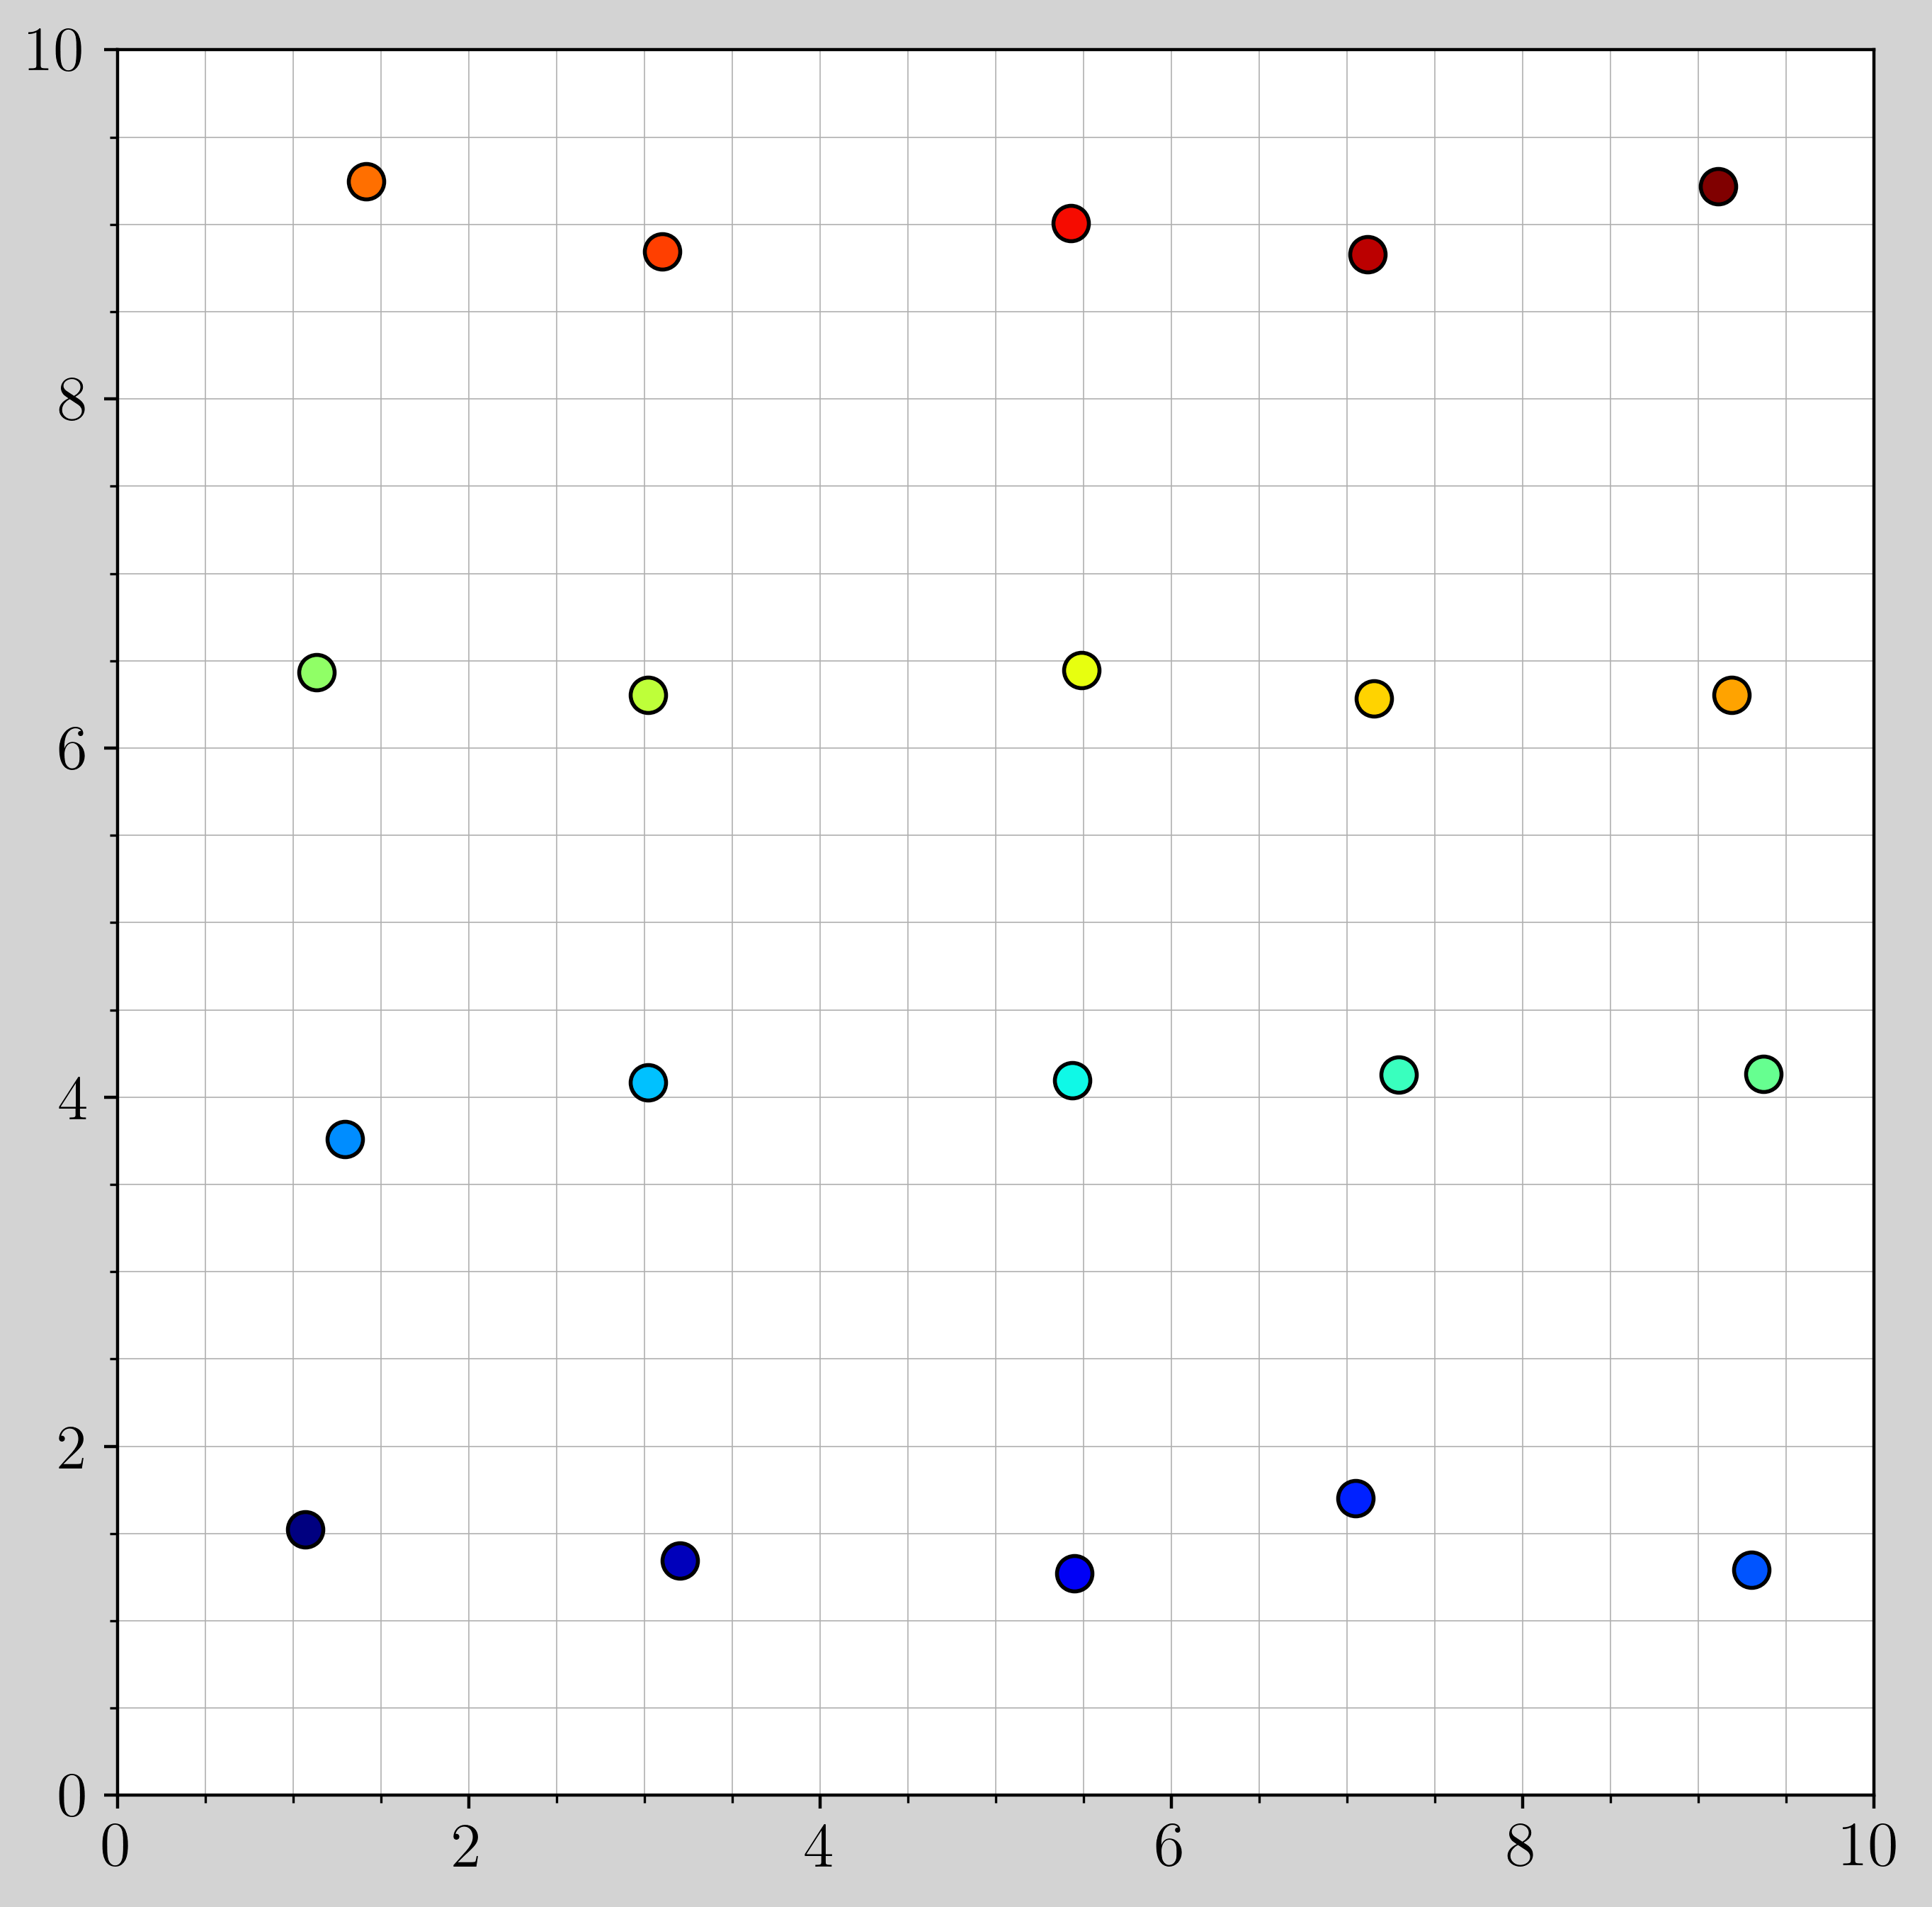
\includegraphics[width=0.4\linewidth]{tarefa-A/posicoes-iniciais.png}
    \caption{Posições iniciais das partículas.}
    \label{fig:posicoes-iniciais-a}
\end{figure}

\begin{figure}[h!]
    \centering 
    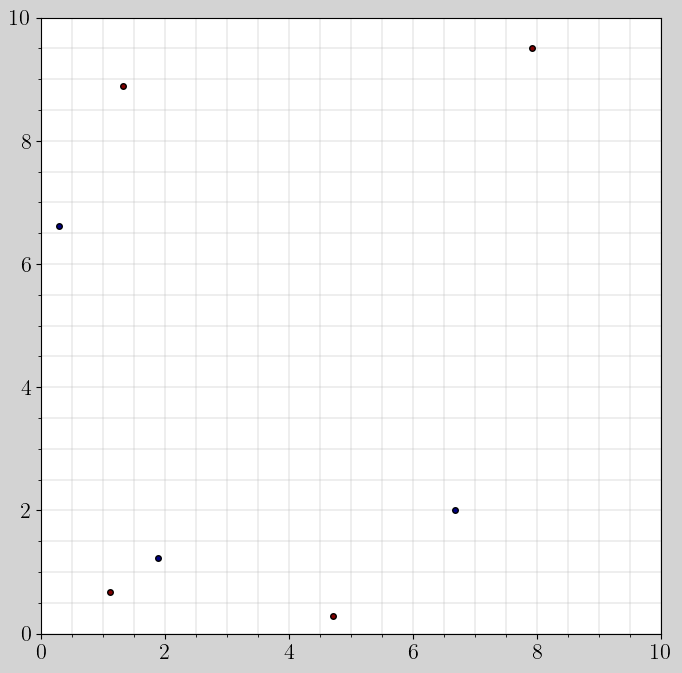
\includegraphics[width=0.4\linewidth]{tarefa-A/posicoes-finais.png}
    \label{fig:posicoes-finais-a}
    \caption{Coordenadas das partículas projetadas à cada $3 \Delta t$.}
\end{figure}

\begin{figure}[h!]
    \centering 
    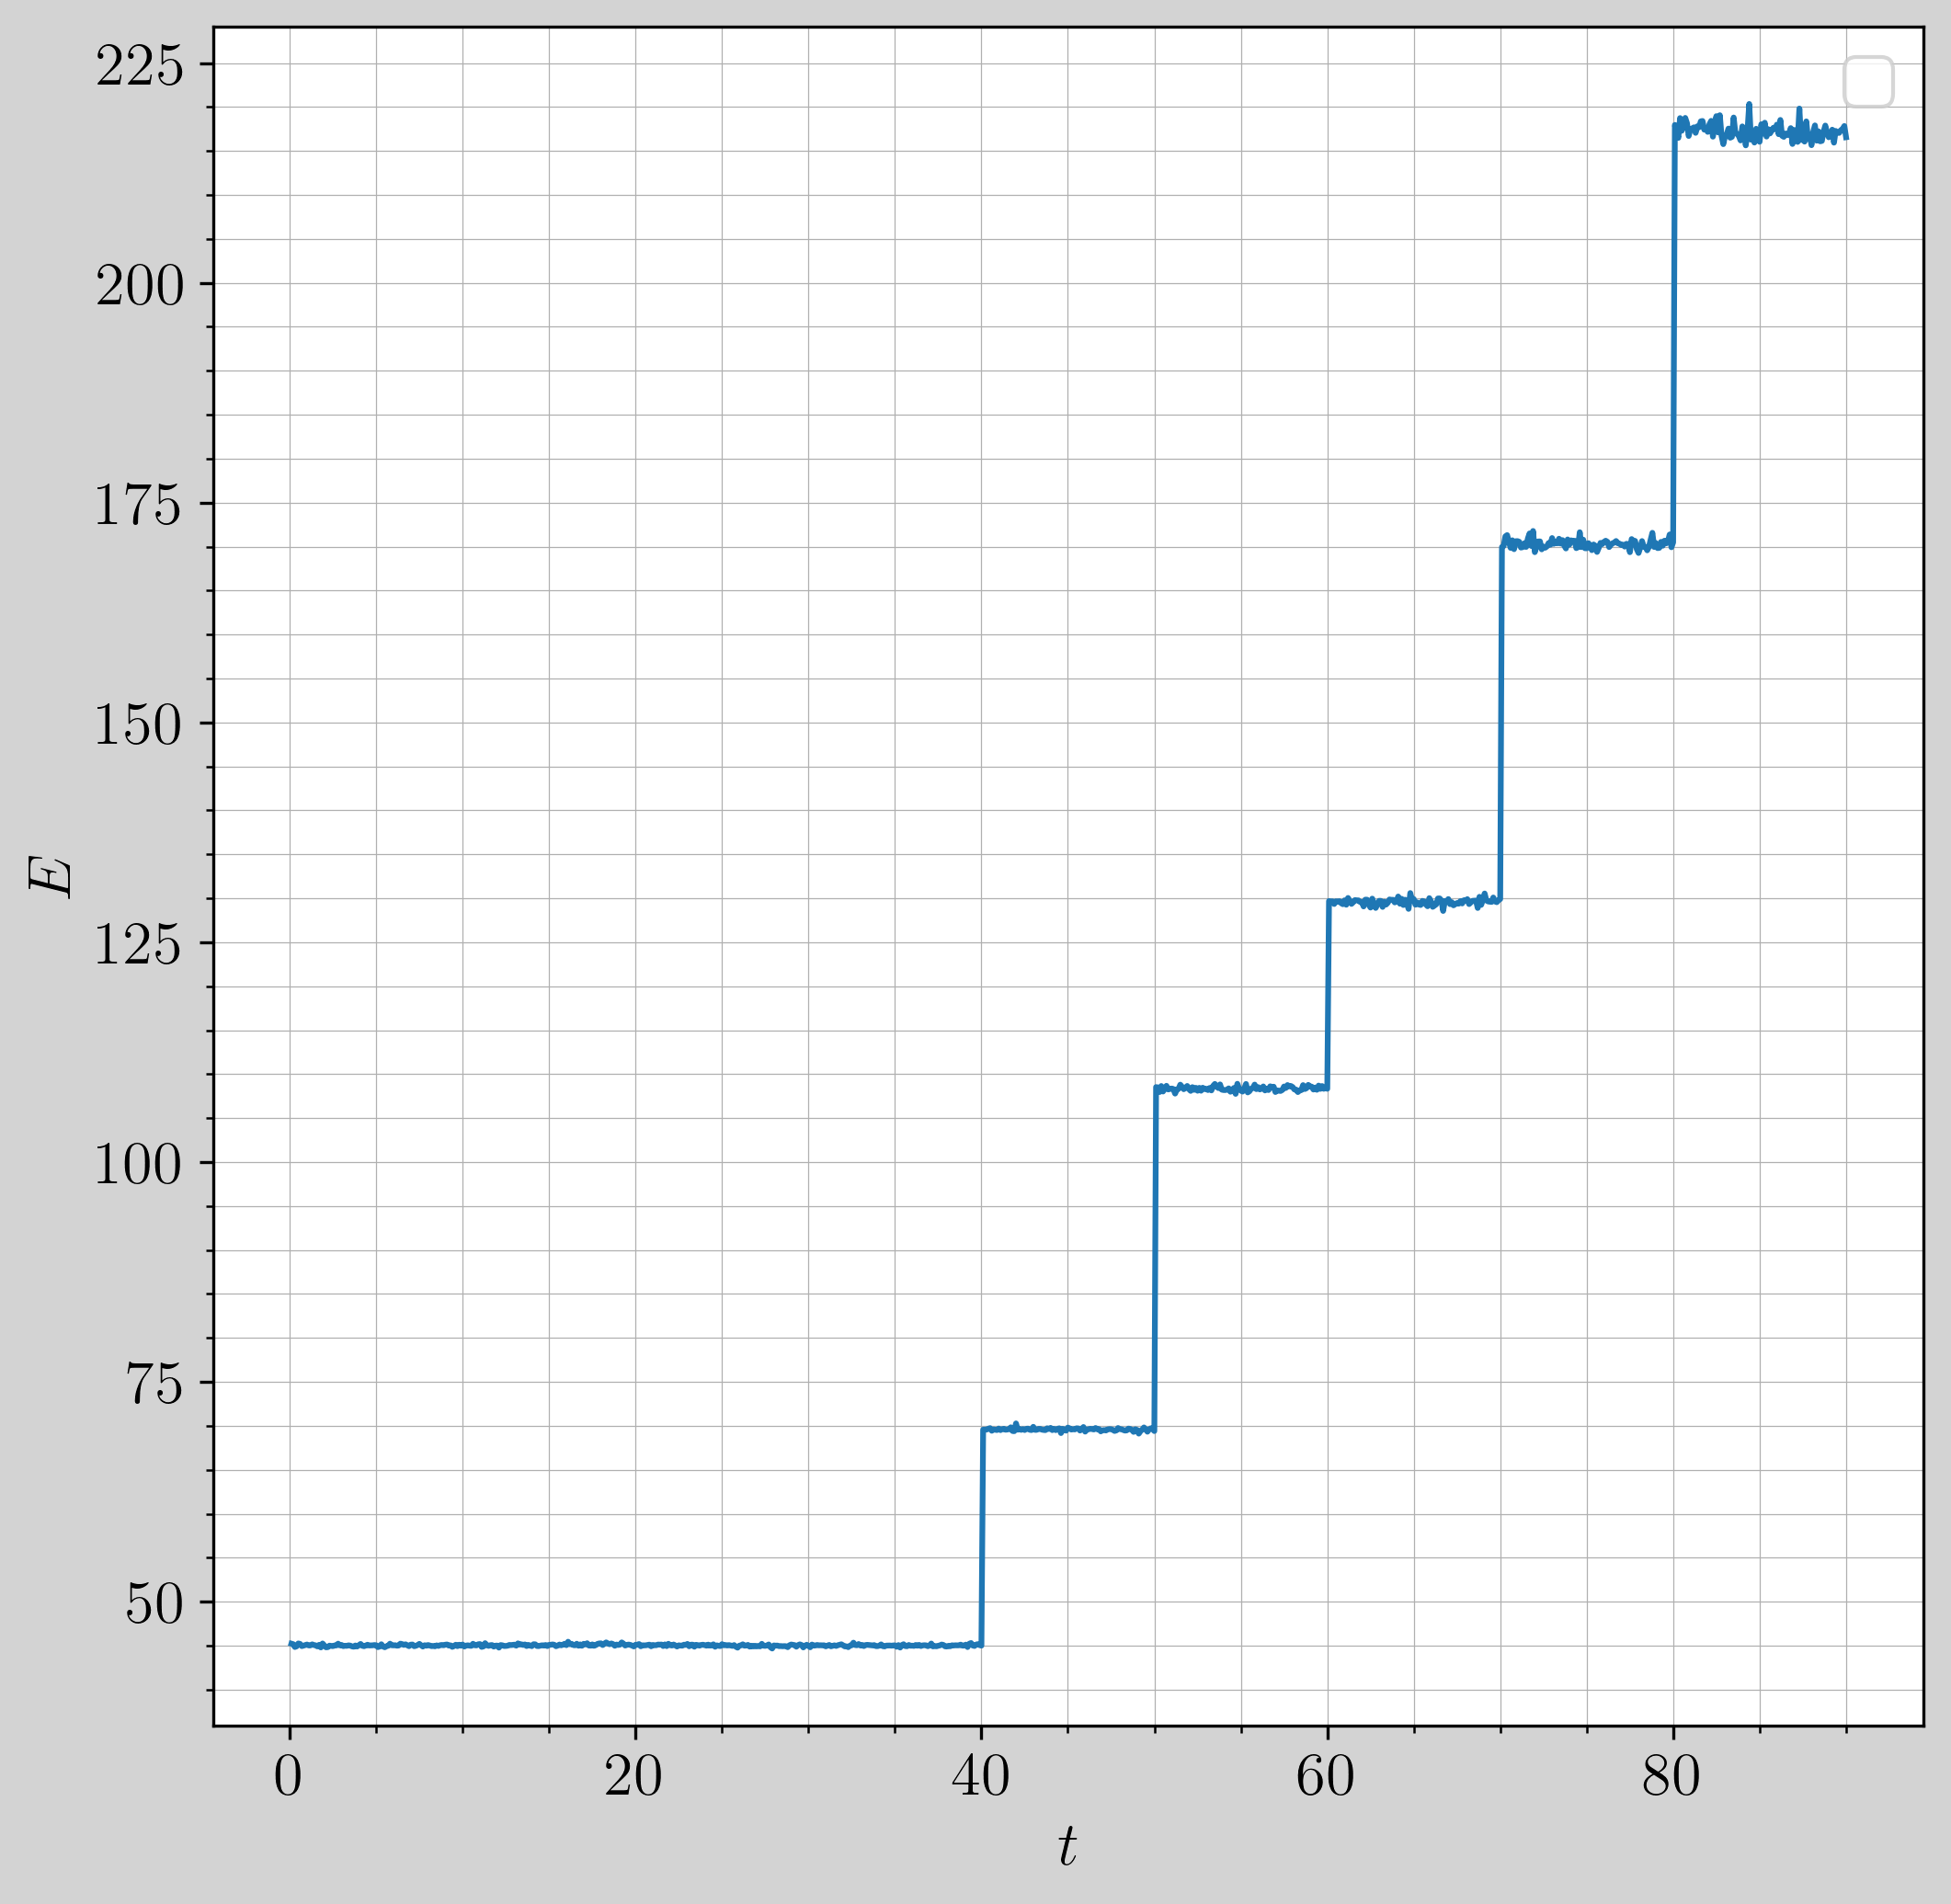
\includegraphics[width=0.4\linewidth]{tarefa-A/energia.png}
    \caption{Energia do sistema à cada $3 \Delta t$.}
    \label{fig:energia_a}
\end{figure}

\clearpage
\subsection*{Código}
O código abaixo está no diretório \verb|tarefa-a/| e contém 
as simulações referentes às tarefas A, B e parte da D.
\begin{minted}{fortran}
    ! Tarefas A, B e parte da D
    implicit real*8(a-h, o-y)
    parameter (pi = acos(-1.e0))
    dimension r_prev(20, 2)
    dimension r_curr(20, 2)
    dimension r_next(20, 2)
    dimension v(20, 2)
    dimension r(20, 20)
    dimension acc(2)
    L = 10
    rL = 10d0
    N = 20

    ! Tarefa A 
    open(unit = 99, file="saidas/tarefa-A/parametros.dat")
    open(unit = 1,  file="saidas/tarefa-A/posicoes-iniciais.dat")
    open(unit = 3,  file="saidas/tarefa-A/evolucao-posicoes.dat")
    ! Tarefa B 
    open(unit = 5,  file="saidas/tarefa-B/velocidades.dat")
    open(unit = 6,  file="saidas/tarefa-B/evolucao-posicoes.dat")
    ! Tarefa D
    open(unit = 9,  file="saidas/tarefa-D/temperatura-b.dat")
    
    dt = 0.02
    v0 = 1.0
    write(99, *) N, L, v0, dt
    close(99)
    ! Defining # rows/columns 
    n_cols = ceiling(sqrt(N*1d0))
    n_rows = ceiling((N*1d0)/(n_cols*1d0)) 
    
    ! Spacing 1/4 
    x_spacing = L/(1d0*n_cols)
    y_spacing = L/(1d0*n_rows)
    spacing = min(x_spacing, y_spacing)/4.0 
    
    ! Centering in the grid
    x_offset = x_spacing / 2.0 
    y_offset = y_spacing / 2.0
    call srand(562369)
    
    k = 1 
    do j = 1, n_rows 
          do i = 1, n_cols 
                r_curr(k, 1) = (i-1)*x_spacing+x_offset
                r_curr(k, 2) = (j-1)*y_spacing+y_offset
                
                r_curr(k, 1) = r_curr(k,1)+(rand())*spacing
                r_curr(k, 2) = r_curr(k,2)+(rand())*spacing
                theta = 2*pi*rand()
                v(k, 1) = v0*cos(theta)
                v(k, 2) = v0*sin(theta)
                
                r_prev(k, 1) = r_curr(k, 1) - v(k, 1) * dt 
                r_prev(k, 2) = r_curr(k, 2) - v(k, 2) * dt 
                k=k+1
          end do 
    end do

    do i = 1, N
          write(1, *) r_curr(i, 1), r_curr(i, 2) 
          write(3, *) 0d0, r_curr(i,1), r_curr(i, 2)
    end do
    close(1)

    DB = 1.0
    ! Dynamics 
    do k = 1, 5000

          t = k * dt 

          acc(1) = 0d0 
          acc(2) = 0d0

          do i = 1, N 
                acc(1) = 0d0 
                acc(2) = 0d0
                do j = 1, N 
                      if(i /= j) then
                           call compute_acc(N,i,j,L,r_curr,acc,r)
                      end if
                end do 
                ! UPDATE POSITIONS
                r_next(i,1) = 2*r_curr(i,1)-r_prev(i,1)+acc(1)*(dt**2)
                r_next(i,2) = 2*r_curr(i,2)-r_prev(i,2)+acc(2)*(dt**2) 

                ! APPLY PBC
                r_next(i,1) = mod(r_next(i,1)+rL, rL)
                r_next(i,2) = mod(r_next(i,2)+rL, rL)

                delta_r_x = delta_pbc(r_next(i,1),r_prev(i,1),L)
                delta_r_y = delta_pbc(r_next(i,2),r_prev(i,2),L)

                ! UPDATE VELOCITIES using adjusted displacements
                v(i, 1) = delta_r_x / (2 * dt)
                v(i, 2) = delta_r_y / (2 * dt)
          end do

          r_prev(:, 1) = r_curr(:, 1)
          r_prev(:, 2) = r_curr(:, 2)
          
          r_curr(:, 1) = r_next(:, 1)
          r_curr(:, 2) = r_next(:, 2)
          
          if(k < 200) then 
                E = 0d0
                call compute_energy(N, L, v, r_curr, E, r)
                write(19,*) k, E
          end if

          ! TAREFA A 
          if(mod(k, 3) == 0 .and. k < 400) then
                do i = 1, N 
                      write(3,*) k, r_curr(i,1),r_curr(i, 2)
                end do
          end if

          ! Tarefa B & D 
          if(mod(k, 20) == 0) then
                do i = 1, N
                      v_mag = sqrt(v(i,1)**2+v(i,2)**2)
                      write(5,*) k, v_mag, v(i,1), v(i,2)
                      write(9,*) .5d0 * v_mag**2
                      write(6,*) k, r_curr(i,1),r_curr(i, 2)
                end do
          end if
    end do
    close(3)
    close(5)
    close(6)
    close(9)
    close(15) 

    end
    ! Submodules for molecular dynamic simulations
    ! Velocity delta 
    function delta_pbc(r_next, r_prev,L)
          implicit real*8(a-h, o-y)
          delta_pbc = r_next - r_prev
          delta_pbc = delta_pbc - L * nint(delta_pbc / L)
    end function delta_pbc

    subroutine initialize_particles(N, L, r_curr,r_prev, v, v0)
          implicit real*8(a-h, o-y)
          dimension r_prev(20, 2)
          dimension r_curr(20, 2)
          dimension v(20, 2)
         
          ! Defining # rows/columns 
          n_cols = ceiling(sqrt(N*1d0))
          n_rows = ceiling((N*1d0)/(n_cols*1d0)) 
          
          ! Spacing 1/4 
          x_spacing = L/(1d0*n_cols)
          y_spacing = L/(1d0*n_rows)
          spacing = min(x_spacing, y_spacing)/4.0 
          
          ! Centering in the grid
          x_offset = x_spacing / 2.0 
          y_offset = y_spacing / 2.0
          call srand(562369)

          k = 1 
          do j = 1, n_rows 
                do i = 1, n_cols 
                      r_curr(k, 1) = (i-1)*x_spacing+x_offset
                      r_curr(k, 2) = (j-1)*y_spacing+y_offset
                      
                      r_curr(k, 1) = r_curr(k,1)+(rand())*spacing
                      r_curr(k, 2) = r_curr(k,2)+(rand())*spacing

                      theta = 2*pi*rand()
                      v(k, 1) = v0*cos(theta)
                      v(k, 2) = v0*sin(theta)
                      
                      r_prev(k, 1) = r_curr(k, 1) - v(k, 1) * dt 
                      r_prev(k, 2) = r_curr(k, 2) - v(k, 2) * dt 
                      k=k+1
                end do 
          end do
    end subroutine initialize_particles

    ! Updates acceleration a = ax, ay 
    ! between particle i and all others
    subroutine compute_acc(N,i,j,L,r_curr,acc, r)
          implicit real*8(a-h, o-y)
          dimension r_curr(20, 2)
          dimension acc(2)
          dimension r(20, 20)
          epsilon = 1e-3

          dx = r_curr(i, 1) - r_curr(j, 1)
          dy = r_curr(i, 2) - r_curr(j, 2)

          dx = dx - L * nint(dx / L)
          dy = dy - L * nint(dy / L)

          r_ij = sqrt(dx**2 + dy**2)
          
          r(i, j) = r_ij 
          r(j, i) = r_ij

          if(r_ij > epsilon .and. r_ij <= 3d0) then 
                F = 24.0 * (2d0/r_ij**13 - 1d0/r_ij**7)
                acc(1) = acc(1) + F * dx / r_ij 
                acc(2) = acc(2) + F * dy / r_ij
          end if 
    end subroutine compute_acc

    subroutine compute_energy(N, L, v, r_curr, E, r)
          implicit real*8(a-h, o-y)
          dimension v(20, 2)
          dimension r_curr(20, 2)
          dimension r(20, 20)
          
          epsilon = 1e-3
          Tk = 0d0
          do i = 1, N
              Tk = Tk + 0.5 * (v(i, 1)**2 + v(i, 2)**2)
          end do
          U = 0d0
          do i = 1, N
            do j = i + 1, N
                r_ij = r(i, j)

                if (r_ij > epsilon .and. r_ij <= 3d0) then
                    U = U + 4 * (r_ij**(-12) - r_ij**(-6))
                end if
            end do
          end do
          E = Tk + U
    end subroutine
\end{minted}
\clearpage
%\clearpage

\section{Tarefa B - \emph{Processos de recozimento e têmpera}}
\begin{align}
    P(v) &\sim \frac{v^2}{K_B T} \exp \left( - \frac{m v^2}{2K_B T} \right)  \\ 
    P(v_x) &\sim \frac{1}{\sqrt{K_B T}}\exp \left( - \frac{m v_x^2}{2K_B T} \right)\\
    P(v_y) &\sim \frac{1}{\sqrt{K_B T}}\exp \left( - \frac{m v_y^2}{2K_B T} \right)
\end{align}





\begin{figure}[h!]
    \centering
    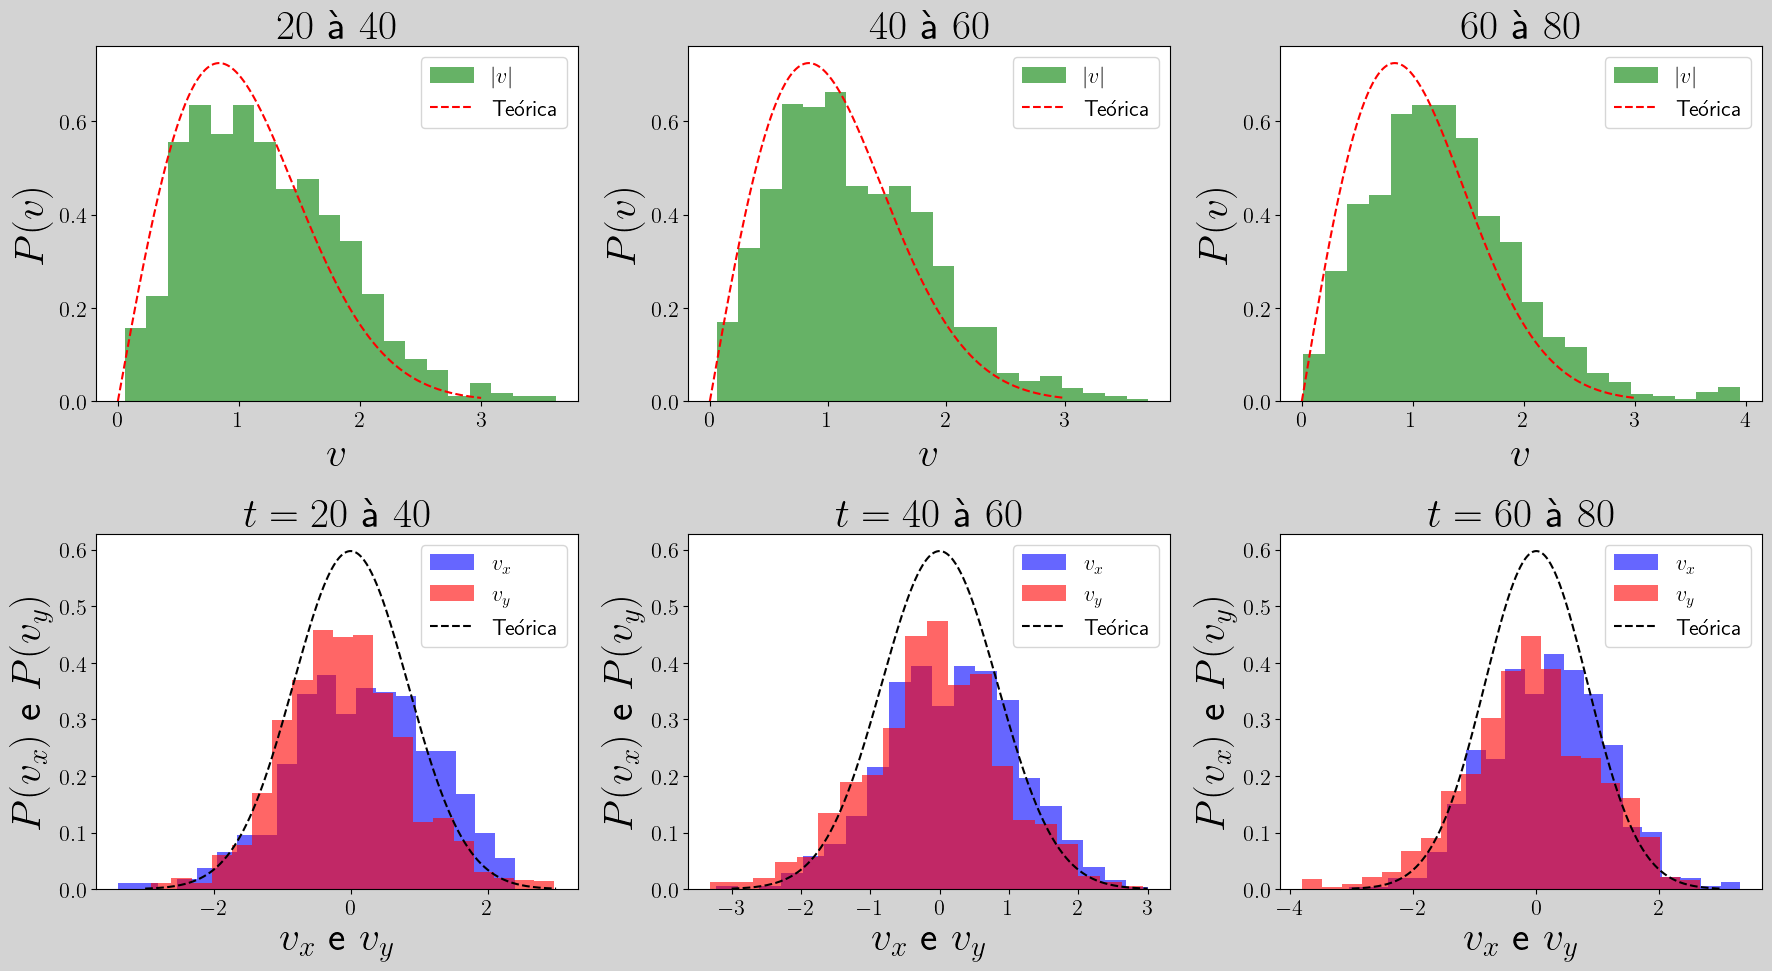
\includegraphics[width=0.7\linewidth]{tarefa-B/distribuicoes-b.png}
    \caption{Distribuição da velocidade, magnitude e componentes em intervalos $t=20-40$, $t=40-60$ e $t=60-80$.}
    \label{fig:distribuicoes-velocidade-b}
\end{figure}


Além disso há um gif para essa simulação.

\clearpage
%\clearpage

\section{Tarefa C - \emph{Loop térmico}}
\subsection{C.1 - Histerese }
Segue abaixo a implementação da simulção de histerese:
\begin{minted}{fortran}
            open(1, file="saidas/tarefa-3/saida-tarefa-C1-L60-DB1.dat")
            open(2, file="saidas/tarefa-3/saida-tarefa-C1-L60-DB2.dat")

            open(3, file="saidas/tarefa-3/saida-tarefa-C1-L80-DB1.dat")
            open(4, file="saidas/tarefa-3/saida-tarefa-C1-L80-DB2.dat")

            open(5, file="saidas/tarefa-3/saida-tarefa-C1-L100-DB1.dat")
            open(6, file="saidas/tarefa-3/saida-tarefa-C1-L100-DB2.dat")


            call tarefaC1(60, 0.001, 1)
            call tarefaC1(60, 0.0001,  2)

            call tarefaC1(80, 0.001, 3)
            call tarefaC1(80, 0.0001, 4)

            call tarefaC1(100,0.001, 5)
            call tarefaC1(100,0.0001, 6)

            do i = 1, 6
                close(i)
            end do
            end

            subroutine tarefaC1(L_real, dbeta, f_name)
                implicit integer(f-f)
            !           Tarefa B - Recozimento e quenching
                implicit real(j-j, m-m)
                parameter(L = 100)
                dimension exps(-4:4)
                byte lattice(1:L, 1:L)

                ! periodic boundary conditions
                dimension ipbc(0:L+1)

                do i = 1, L_real
                    ipbc(i) = i
                end do  

                ipbc(0) = L_real
                ipbc(L_real+1) = 1

                N = L_real * L_real

                mag = 0.0d0

                call srand(96312)
                ! b = 0
                call initialize_random_lattice(lattice,  L_real, L_real)

                call total_magnetization(lattice, mag, L_real)

                ! initial energy
                E = H_0(lattice, ipbc, L_real)

                beta = 0.0

                write(f_name, *) 0, beta,  mag, E/N

                imax = int(1.75 / dbeta) + 1 

                do i = 1, imax

                    call define_exponentials(exps, beta)

                    if(i < imax/ 2) then 
                        beta = beta + dbeta 
                    else
                        beta = beta - dbeta 
                    end if  

                    do k = 1 , N
                        call flip_spin(lattice,ipbc,exps,E,mag,L_real)
                    end do   

                    write(f_name, *) i, beta, mag, E/N

                end do
            end subroutine tarefaC1
\end{minted}


No gráfico (\ref{fig:c1_dbeta1}) temos o comportamento da energia média por spin na dinâmica do loop
térmico e o gráfico de histerese, isto é, a energia média em relação à $\beta$ para 
variações de $\Delta b = 0,001$. 

\begin{figure}
    \centering
    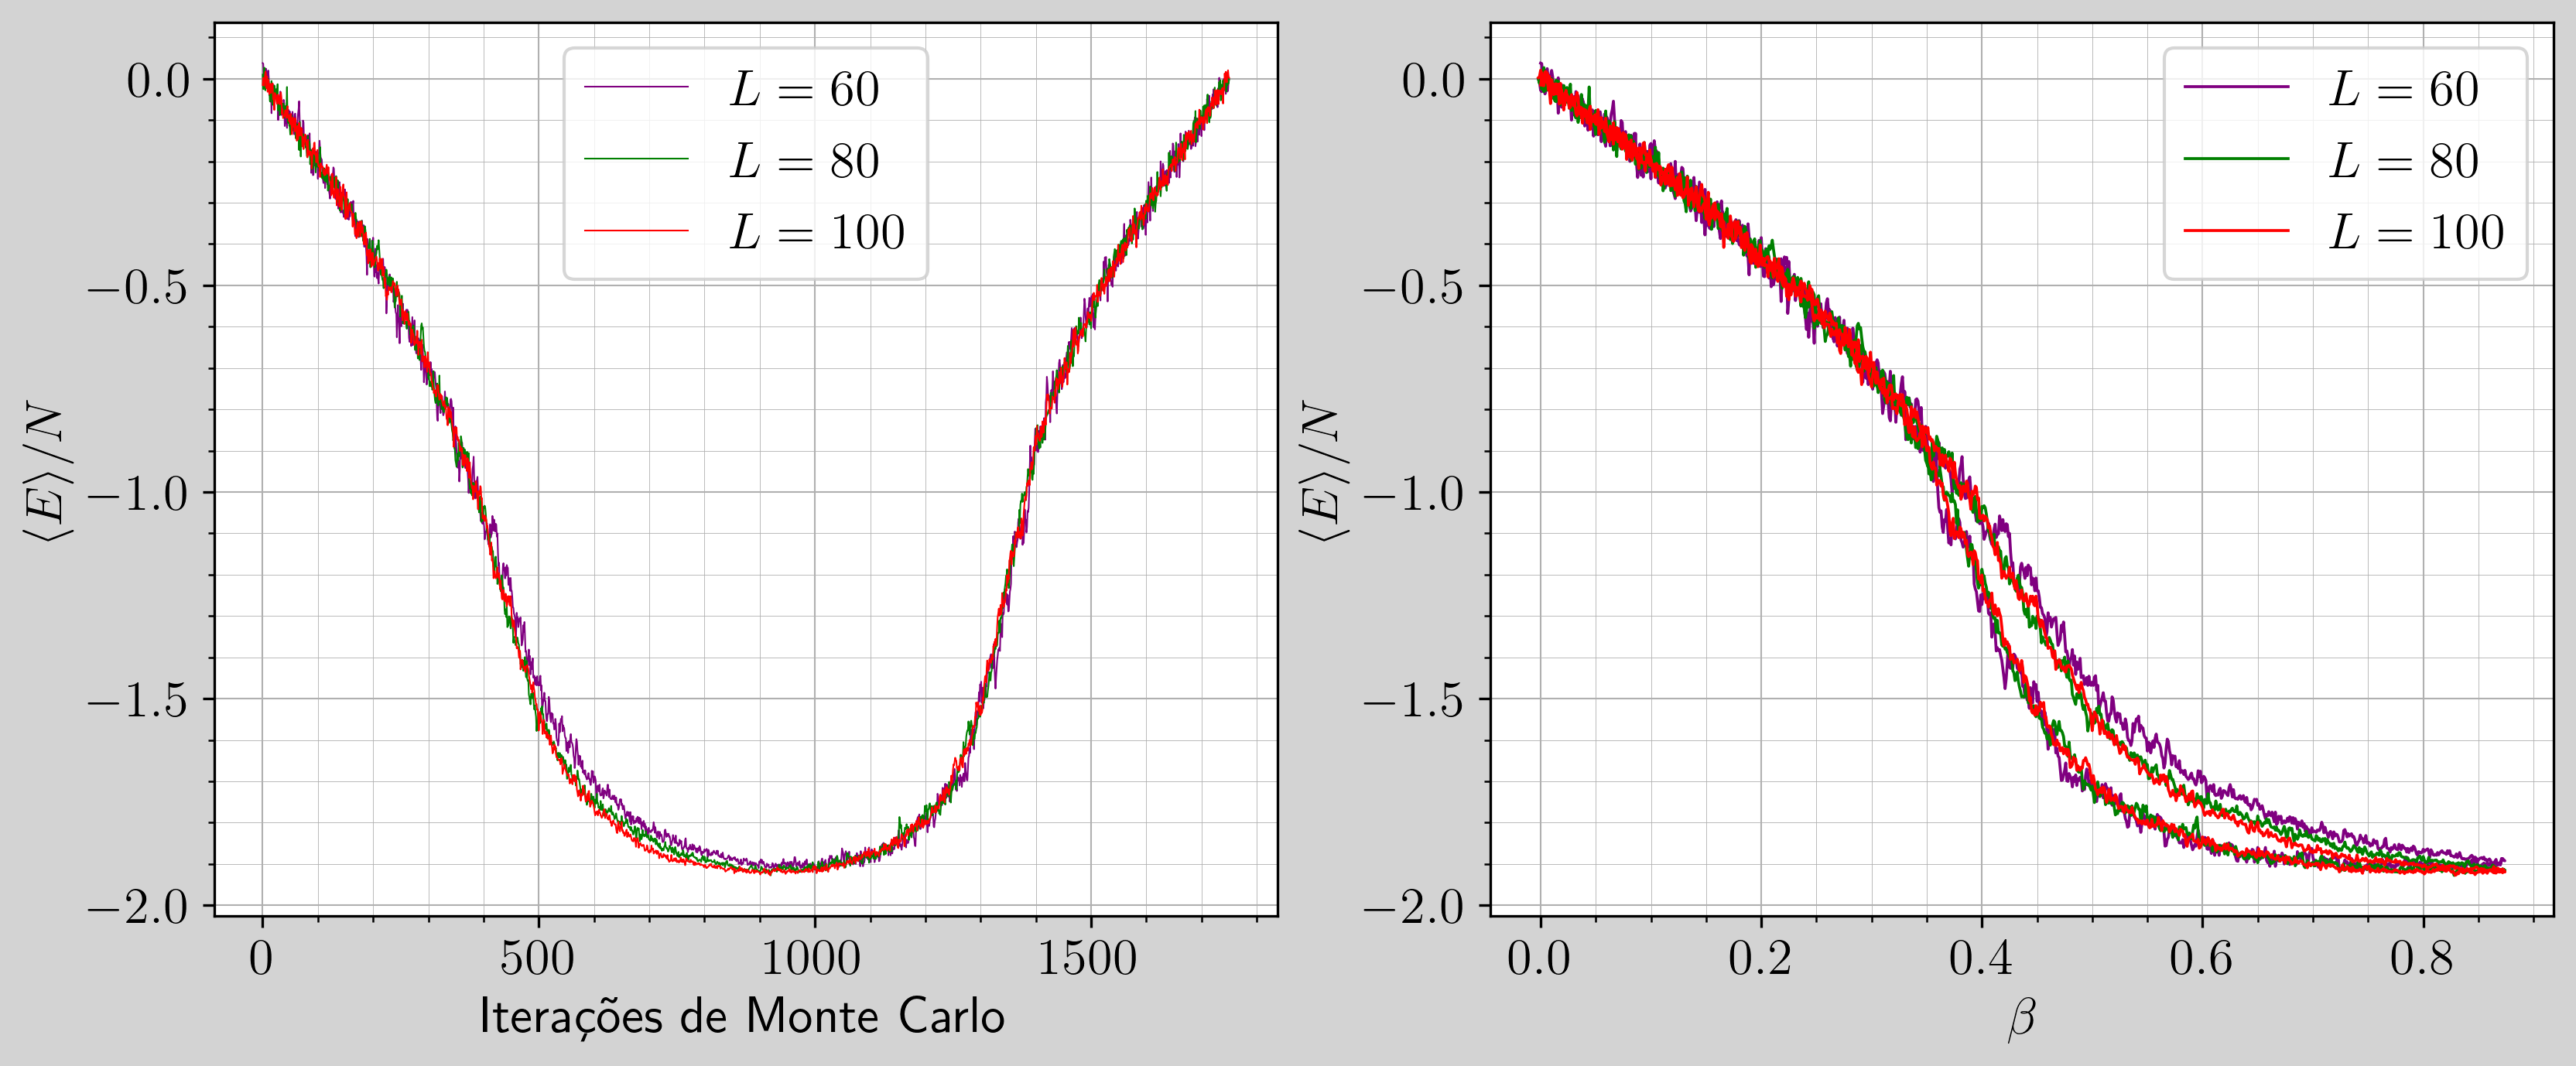
\includegraphics[width=0.8\linewidth]{graficos/tarefa-3/graf-tarefa-C1-delta1.png}
    \caption{À esquerda energia média por spin por iterações de Monte Carlo e à direita em relação à $\beta$.}
    \label{fig:c1_dbeta1}
\end{figure}


A figura (\ref{fig:c1_dbeta2}) equivale a dinâmica como a anterior, mas com uma variação 
$\Delta \beta = 0,0001$, que fornece um resultado com menos flutuações, sobretudo para as redes maiores.

\begin{figure}
    \centering
    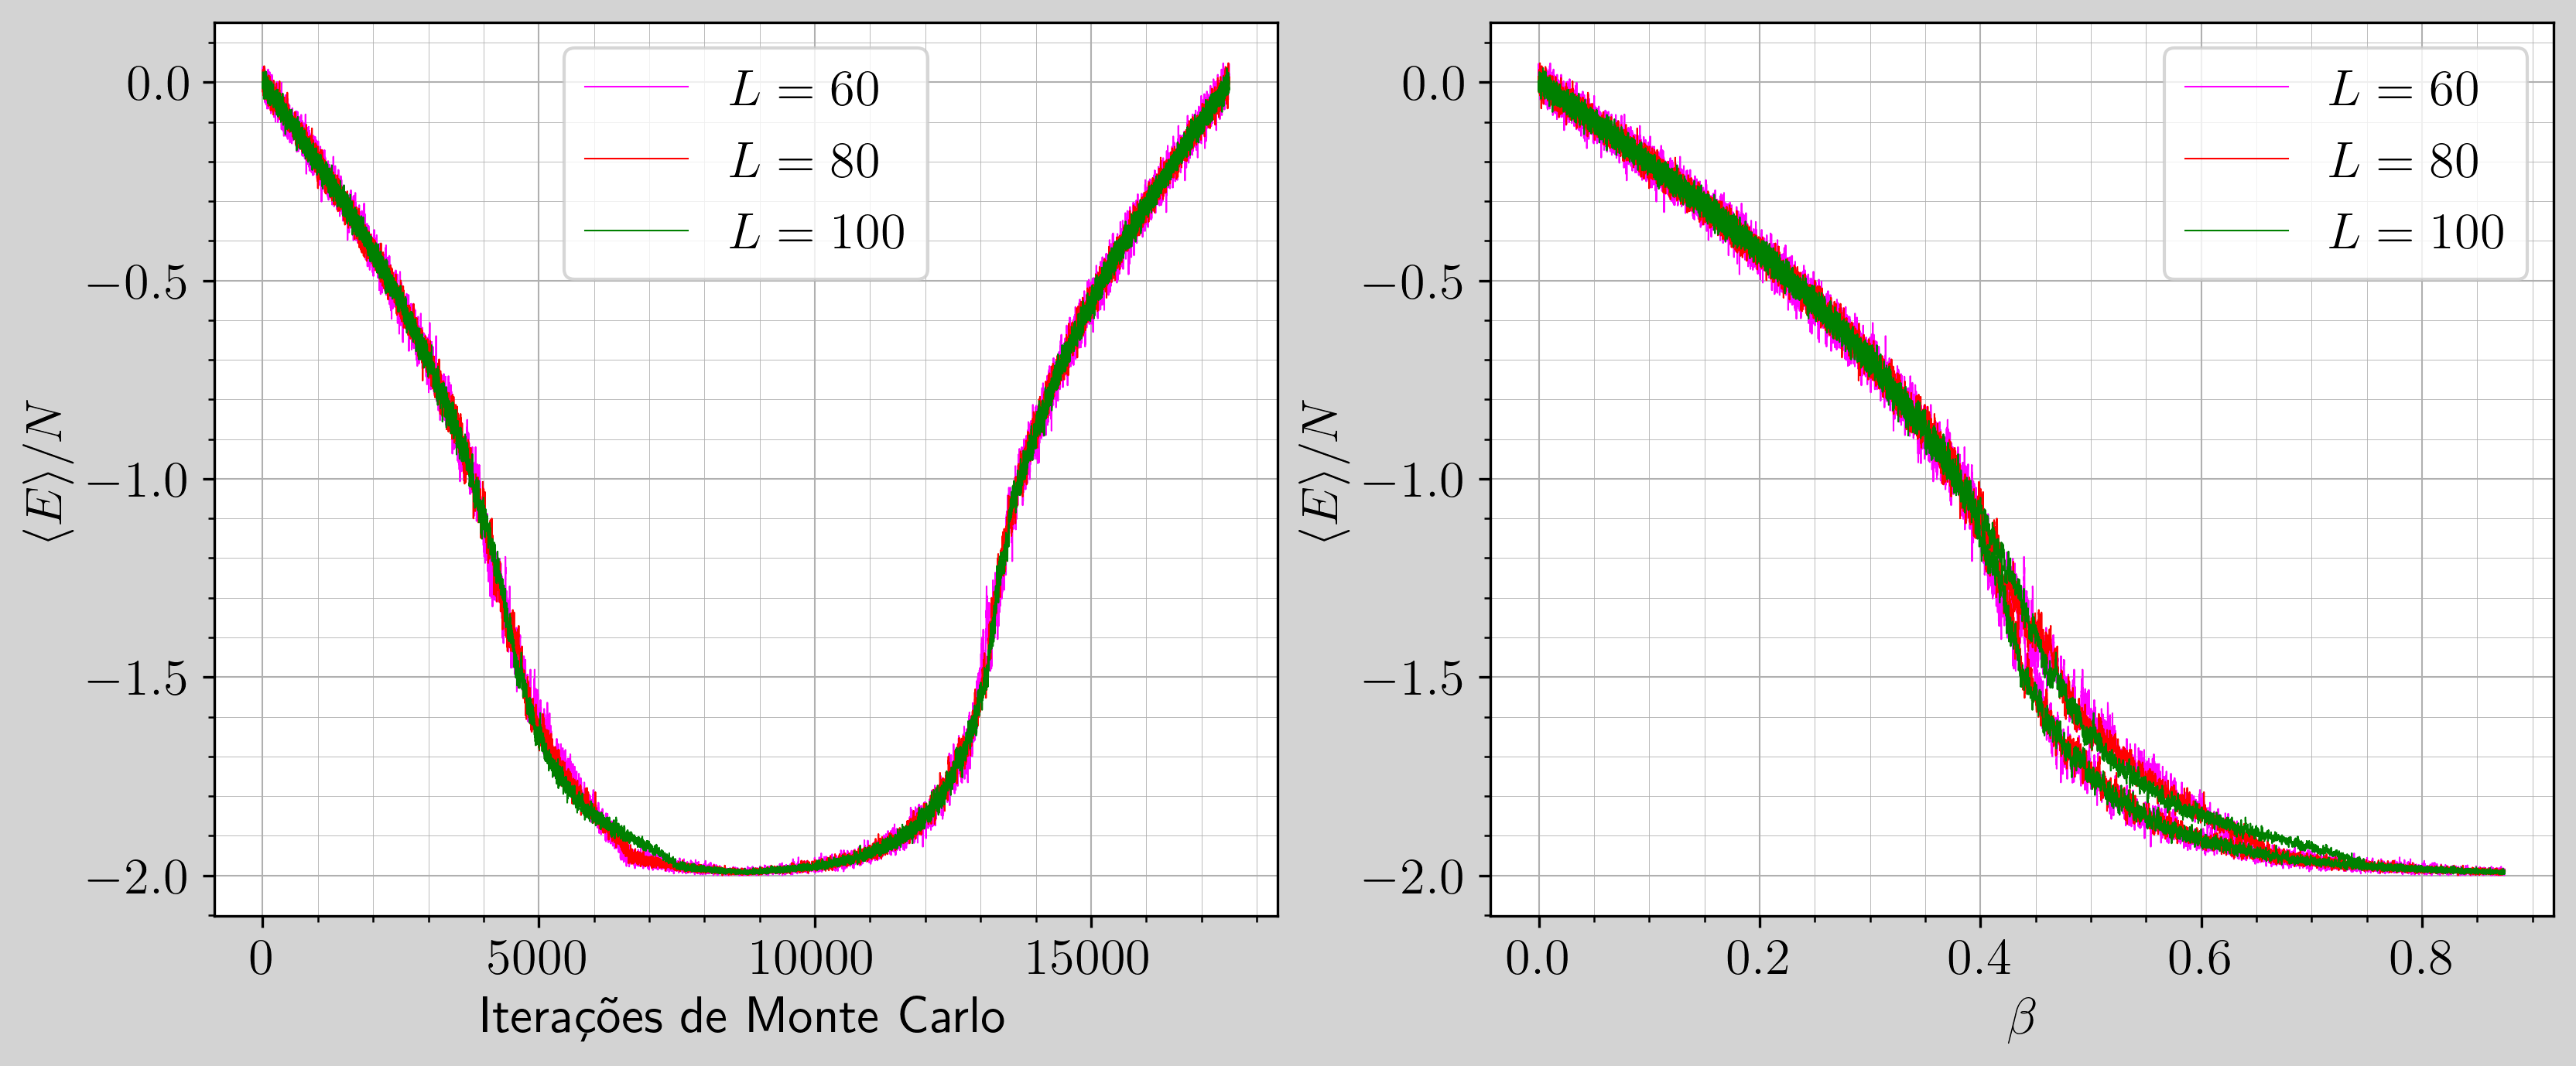
\includegraphics[width=0.8\linewidth]{graficos/tarefa-3/graf-tarefa-C1-delta2.png}
    \caption{À esquerda energia média por spin por iterações de Monte Carlo e à direita em relação à $\beta$.}
    \label{fig:c1_dbeta2}
\end{figure}

Podemos observar nos gráficos que a região de histerese correspondem à um intervalo de $\beta$ entre $0,4$ e 
$0,6$, mas apenas a partir dessas medidas não conseguimos ter uma boa precisão dessa medida.

\subsection{C.2 - Temperatura crítica }


\begin{marginfigure}
    \centering
    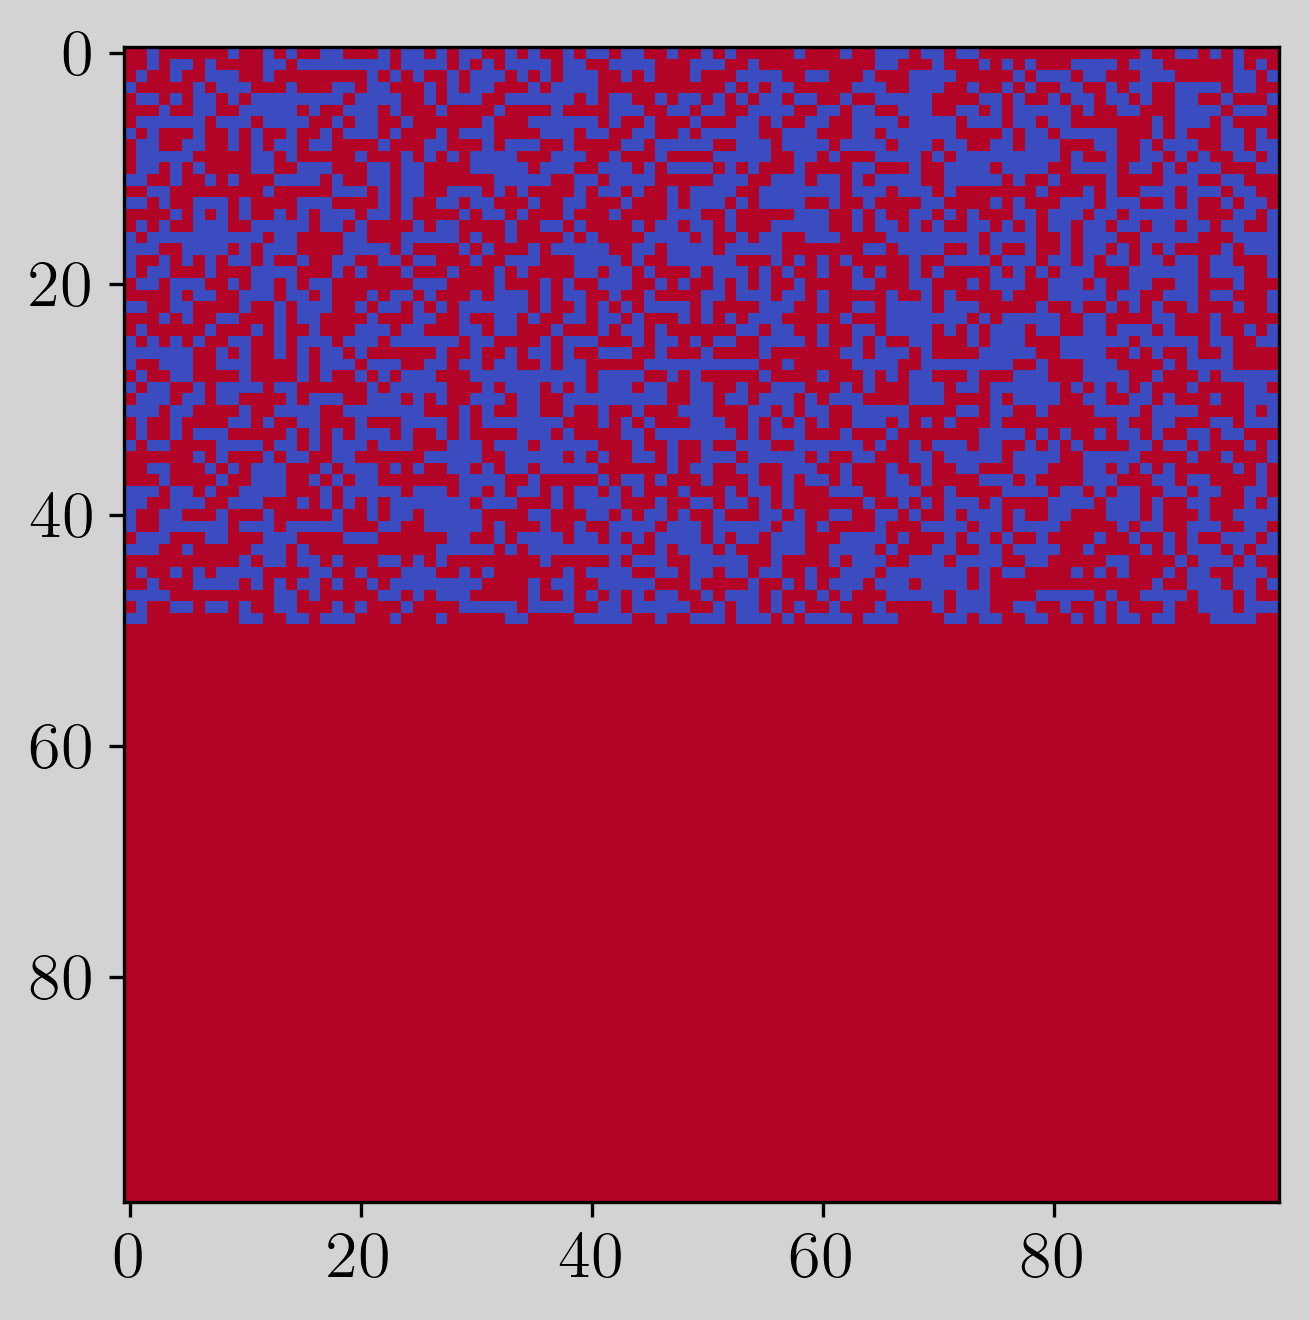
\includegraphics[width=\linewidth]{graficos/tarefa-3/graf-tarefa-C2-conf.png}
    \caption{Configuração inicial para dinâmica utilizada na medida de temperatura crítica.}
    \label{fig:c2_conf_inicial}
\end{marginfigure}


Modificação no código do item anterior: 

\begin{minted}{fortran}

        dimension betas(1:5)
        parameter(betas = (/0.41, 0.44, 0.47, 0.51, 0.55/))

        open(1, file="saidas/tarefa-3/saida-tarefa-C2-L60-b1.dat")
        open(2, file="saidas/tarefa-3/saida-tarefa-C2-L60-b2.dat")
        open(3, file="saidas/tarefa-3/saida-tarefa-C2-L60-b3.dat")
        open(4, file="saidas/tarefa-3/saida-tarefa-C2-L60-b4.dat")
        open(5, file="saidas/tarefa-3/saida-tarefa-C2-L60-b5.dat")

        do i = 1, 5
            call tarefaC2(60, betas(i), i)
            close(1)
        end do

        open(1, file="saidas/tarefa-3/saida-tarefa-C2-L80-b1.dat")
        open(2, file="saidas/tarefa-3/saida-tarefa-C2-L80-b2.dat")
        open(3, file="saidas/tarefa-3/saida-tarefa-C2-L80-b3.dat")
        open(4, file="saidas/tarefa-3/saida-tarefa-C2-L80-b4.dat")
        open(5, file="saidas/tarefa-3/saida-tarefa-C2-L80-b5.dat")

        do i = 1, 5
            call tarefaC2(80, betas(i), i)
            close(1)
        end do

        open(1, file="saidas/tarefa-3/saida-tarefa-C2-L100-b1.dat")
        open(2, file="saidas/tarefa-3/saida-tarefa-C2-L100-b2.dat")
        open(3, file="saidas/tarefa-3/saida-tarefa-C2-L100-b3.dat")
        open(4, file="saidas/tarefa-3/saida-tarefa-C2-L100-b4.dat")
        open(5, file="saidas/tarefa-3/saida-tarefa-C2-L100-b5.dat")

        do i = 1, 5
            call tarefaC2(100, betas(i), i)
            close(1)
        end do
        end
        subroutine tarefaC2(L_real, beta, fname)
!               Tarefa B - Recozimento e quenching
            implicit integer(f-f)
            implicit real(j-j, m-m)
            parameter(L = 100)
            dimension exps(-4:4)
            byte lattice(1:L, 1:L)
            ! periodic boundary conditions
            dimension ipbc(0:L+1)

            do i = 1, L_real
                ipbc(i) = i
            end do  

            ipbc(0) = L_real
            ipbc(L_real+1) = 1

            N = L_real * L_real

            mag = 0.0d0

            call srand(L_real * 392)

            ! half ordered / half random.
            call initialize_lattice(lattice, L_real, L_real)
            call initialize_random_lattice(lattice,  L_real/2, L_real)

            open(99, file = "saidas/tarefa-3/saida-tarefa-C2-conf.dat")
            call write_lattice(lattice, L_real, 99)
            close(99)

            call total_magnetization(lattice, mag, L_real)

            ! initial energy
            E = H_0(lattice, ipbc, L_real)
            dbeta = 0.01
            write(fname, *) 0, E/N
            do i = 1, 3000
                call define_exponentials(exps, beta)
                do k = 1 , N
                    call flip_spin(lattice,ipbc,exps,E,mag,L_real)
                end do   
                write(fname, *) i, E/N
            end do
        end subroutine tarefaC2
\end{minted}


\begin{marginfigure}
    \centering
    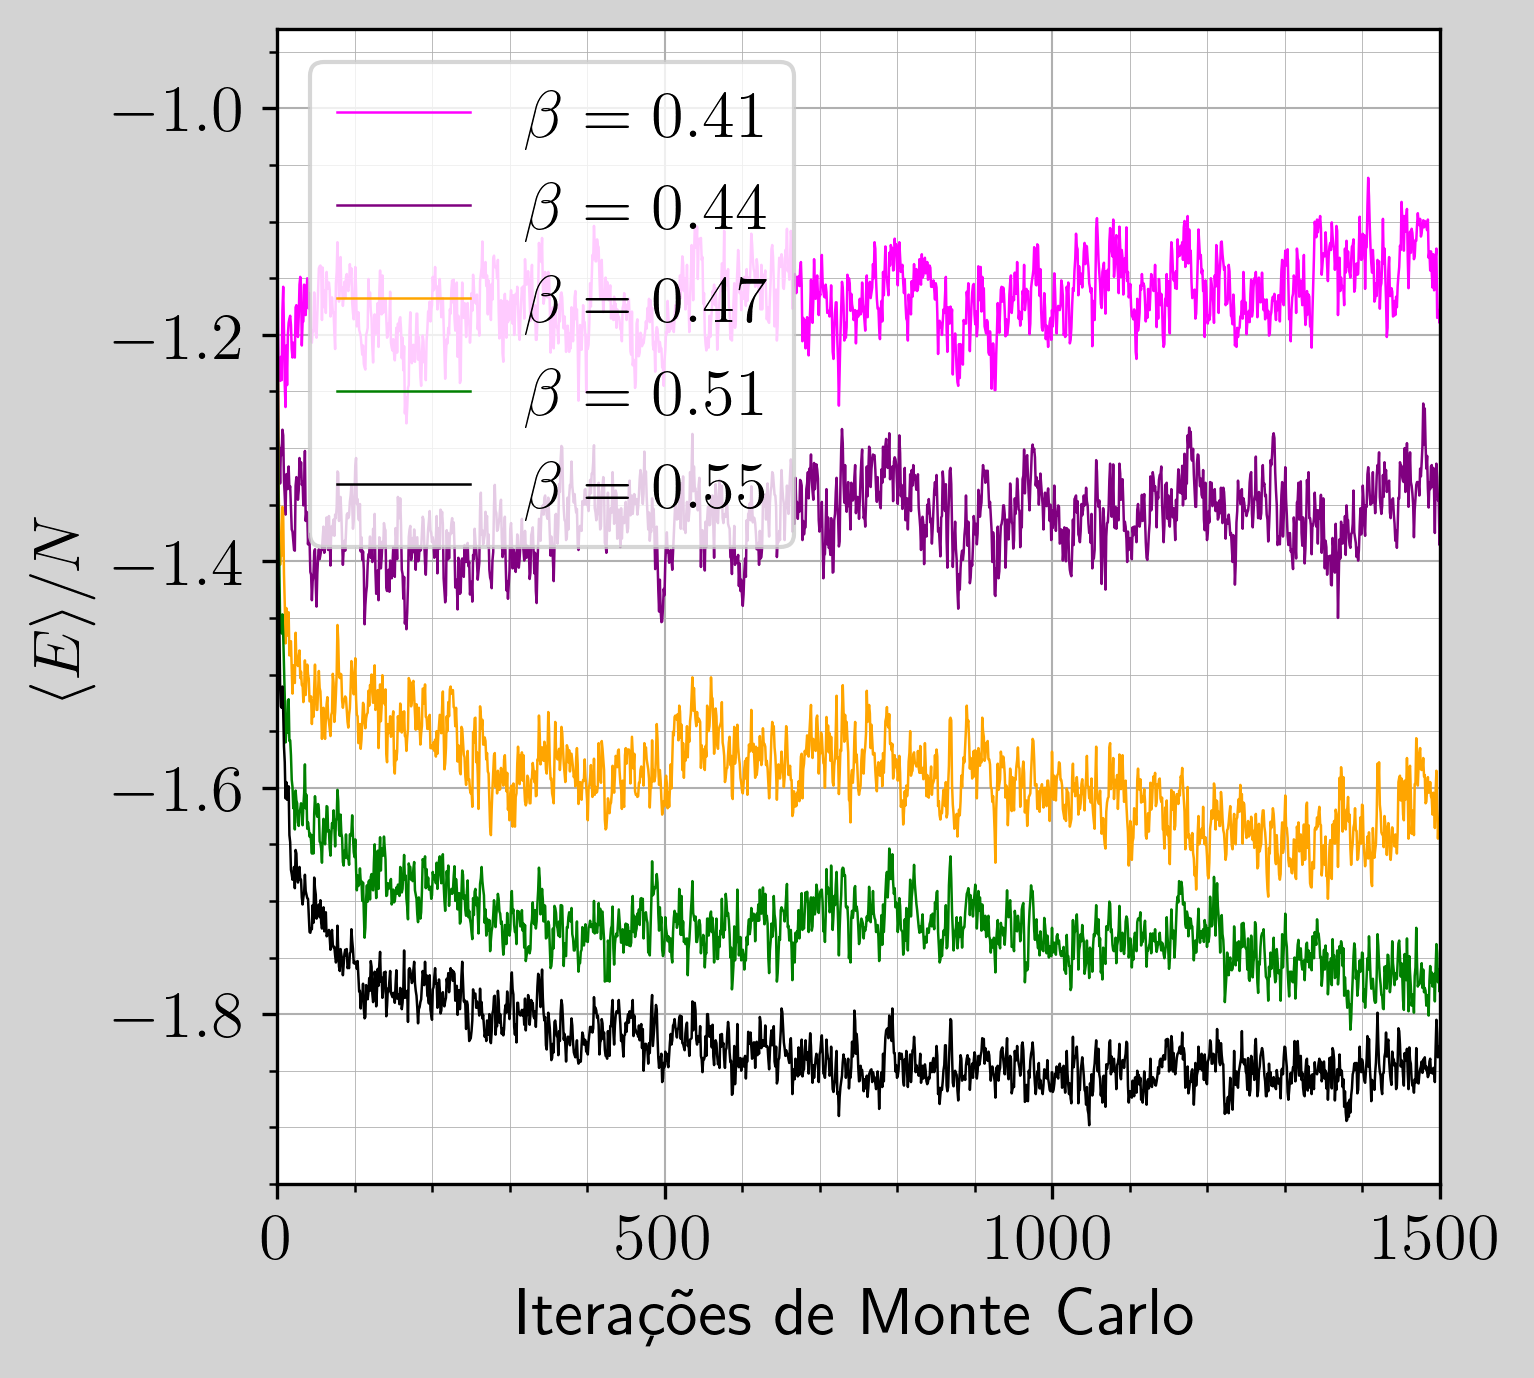
\includegraphics[width=\linewidth]{graficos/tarefa-3/graf-tarefa-C2-L80.png}
    \caption{Dinâmica para L=80.}
    \label{fig:c2_l80}
\end{marginfigure}

Partimos dos resultados do item anterior e tentamos obter a temperatura crítica do modelo. Para isso observamos
a variação de energia no intervalo $\beta$ discutido antes, isto é, $0,4 < \beta < 0.6$. 
A imagem (\ref{fig:c2_conf_inicial}) mostra a configuração inicial do sistema. Foram escolhidos alguns 
valores de $\beta$ para executar a dinâmica de Monte Carlo. 


\begin{marginfigure}
    \centering
    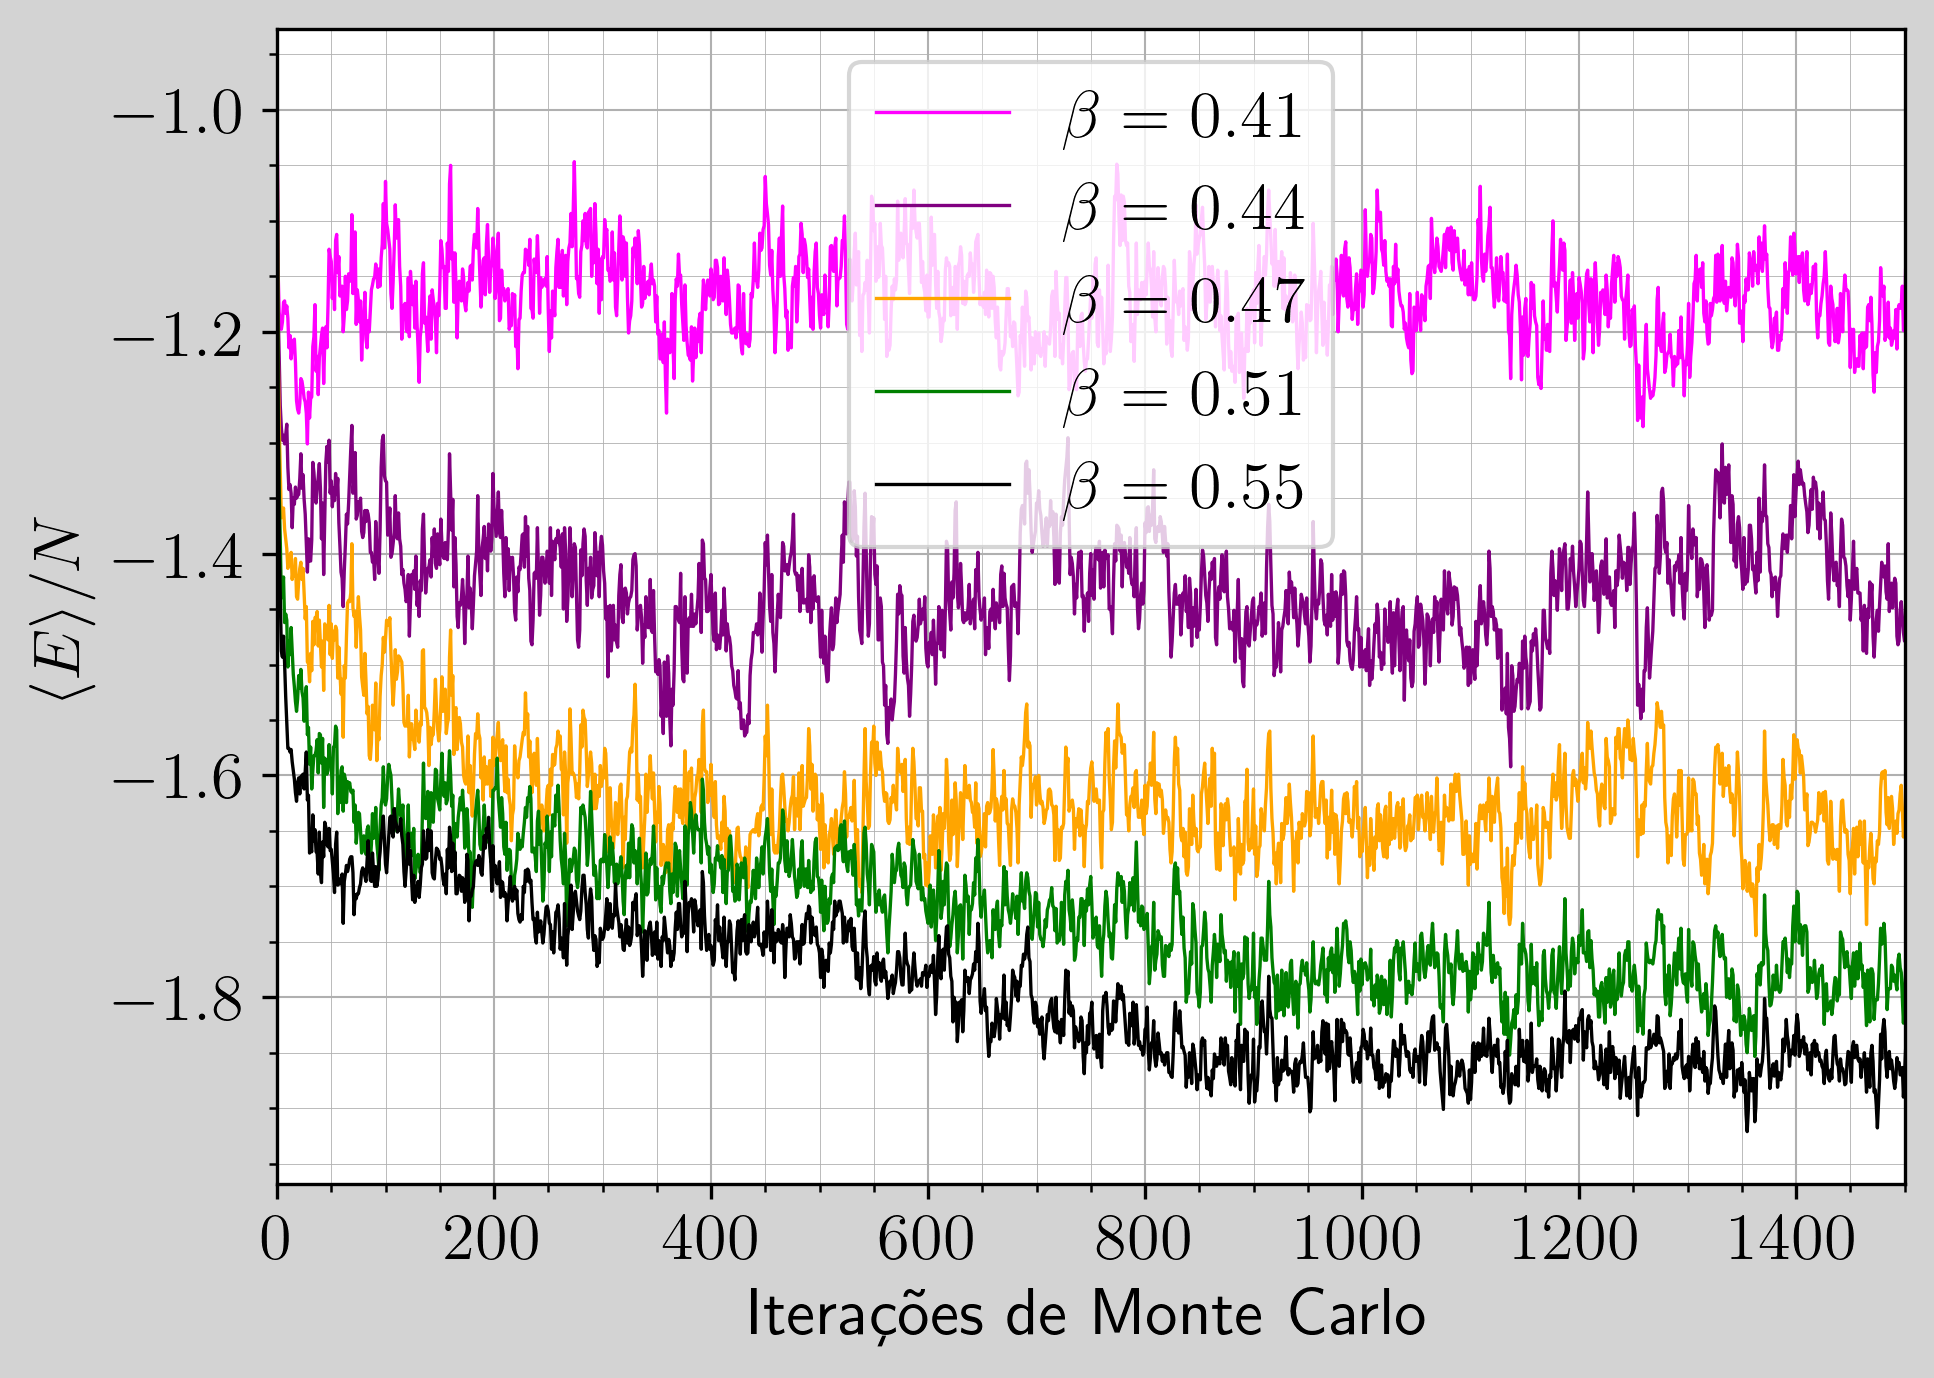
\includegraphics[width=\linewidth]{graficos/tarefa-3/graf-tarefa-C2-L60.png}
    \caption{Dinâmica para L=60.}
    \label{fig:c2_l60}
\end{marginfigure}



Nas figuras (\ref{fig:c2_l60}), (\ref{fig:c2_l80}) e (\ref{fig:c2_l100}) estão 
as evoluções, em um intervalo de passos de Monte Carlo reduzido, da energia média por spin. 

\clearpage
Nota-se que as energias médias por spin sempre partem do mesmo valor no intervalo da histerese e a 
que possui maior variação é a que corresponde à $\beta = 0.44$, esse é o $\beta$ relacionado à temperatura crítica $T_c = 1/\beta_c \approx 2,27$ .

\begin{figure}
    \centering
    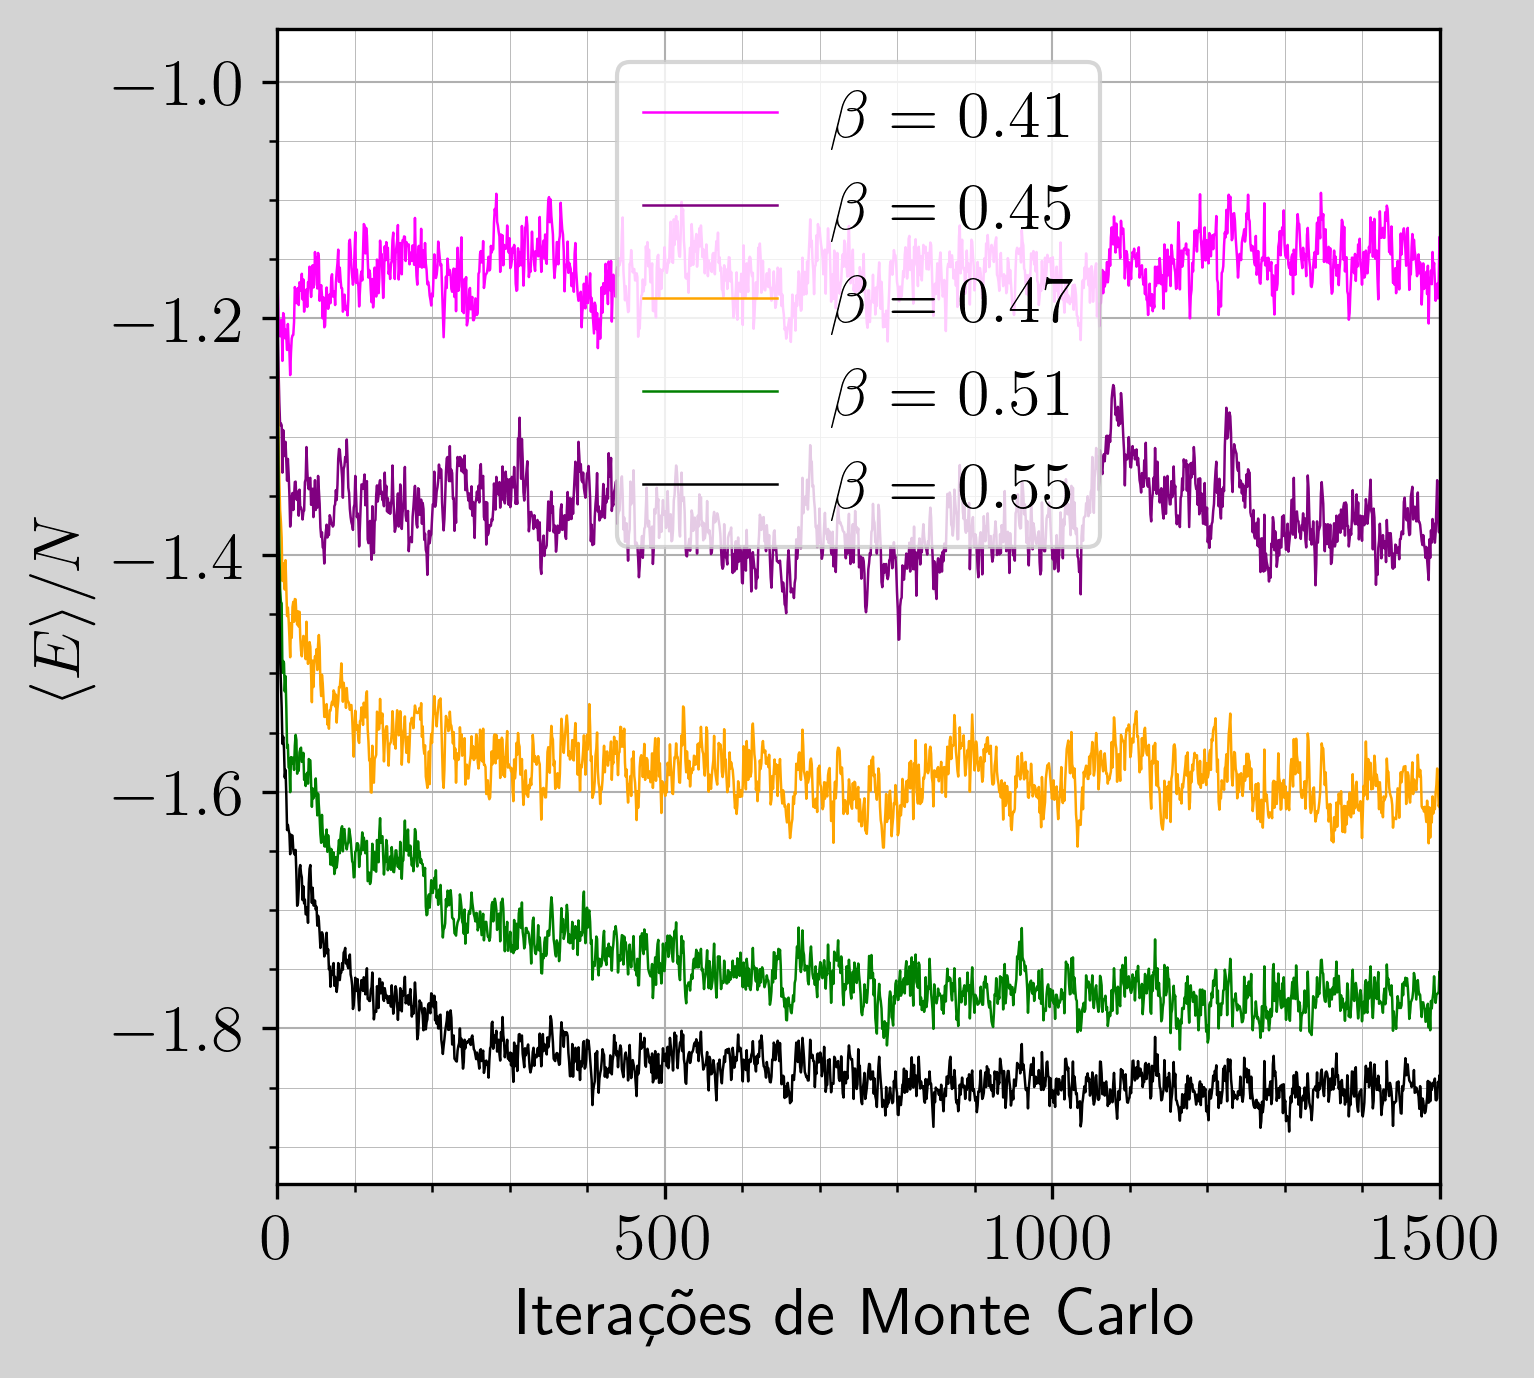
\includegraphics[width=0.5\linewidth]{graficos/tarefa-3/graf-tarefa-C2-L100.png}
    \caption{Dinâmica para L=100.}
    \label{fig:c2_l100}
\end{figure}

Além disso, pela (\ref{eq:calor_especifico}) podemos constatar que esse $\beta_c = 0,44$ também está associado à 
um valor específico crítico no modelo. 
%\clearpage

\section{Tarefa D - \emph{Quebra espontânea de simetria}}
Nessa tarefa o nosso interesse é estudar o fenômeno de quebra espontânea de simetria. 
Queremos mostrar que o tempo que um sistema leva para mudar toda a orientação de magnetização cresce de forma 
exponencial com a dimensão da malha utilizada. 
Para isso foi implementado uma simulação que executa passos de Monte Carlo e contabiliza o intervalo 
de tempo de Monte Carlo que o sistema leva para mudar a magnetização conforme o tamanho $L$ da rede aumenta. 

O código em fortran para essa simulação está abaixo: 

\begin{minted}{fortran}
    implicit integer(f-f)
    implicit real(m-m)
    parameter(L = 100)
    dimension exps(-4:4)
    byte lattice(1:L, 1:L)
    ! periodic boundary conditions
    dimension ipbc(0:L+1)
    ! this or using mod
    open(unit=1, file="saidas/tarefa-4/saida-tarefa-D.dat")
    open(unit=2, file="saidas/tarefa-4/saida-tarefa-MAG_T.dat")
    beta = 0.5
    call define_exponentials(exps, beta)
    do L_real = 4, 10
        print *, "L = ", L_real 
        call srand(3519) ! /L_real+1)
        N = L_real * L_real
        ! setting ipbc
        do i = 1, L_real
            ipbc(i) = i
        end do  
        ipbc(0) = L_real
        ipbc(L_real+1) = 1
        mag = 0.0e0
        call initialize_random_lattice(lattice, L_real, L_real)
        call total_magnetization(lattice, mag, L_real)
        n_inversions = 10000
        n_curr = 0
        n_time = 0
        do while(n_curr < n_inversions) 
            mag_prev = mag
            do i = 1, N
                call flip_spin(lattice, ipbc, exps, E, mag, L_real)
            end do
            n_time = n_time + 1
            ! Fazer o gráfico da magnetização aqui.
            if(mag_prev * mag < 0) then 
                t_mean = t_mean + n_time
                n_time = 0
                n_curr = n_curr + 1
            end if
        end do
        write(2, *) t_mean, mag
        t_mean = t_mean / n_inversions
        write(1, *) L_real, t_mean
    end do
    close(1)
    end
\end{minted}

Podemos ver pela figura(\ref{fig:d_graficos}) que o intervalo cresce de forma exponencial com 
o tamanho $L$ da malha: 

\begin{figure}
    \centering
    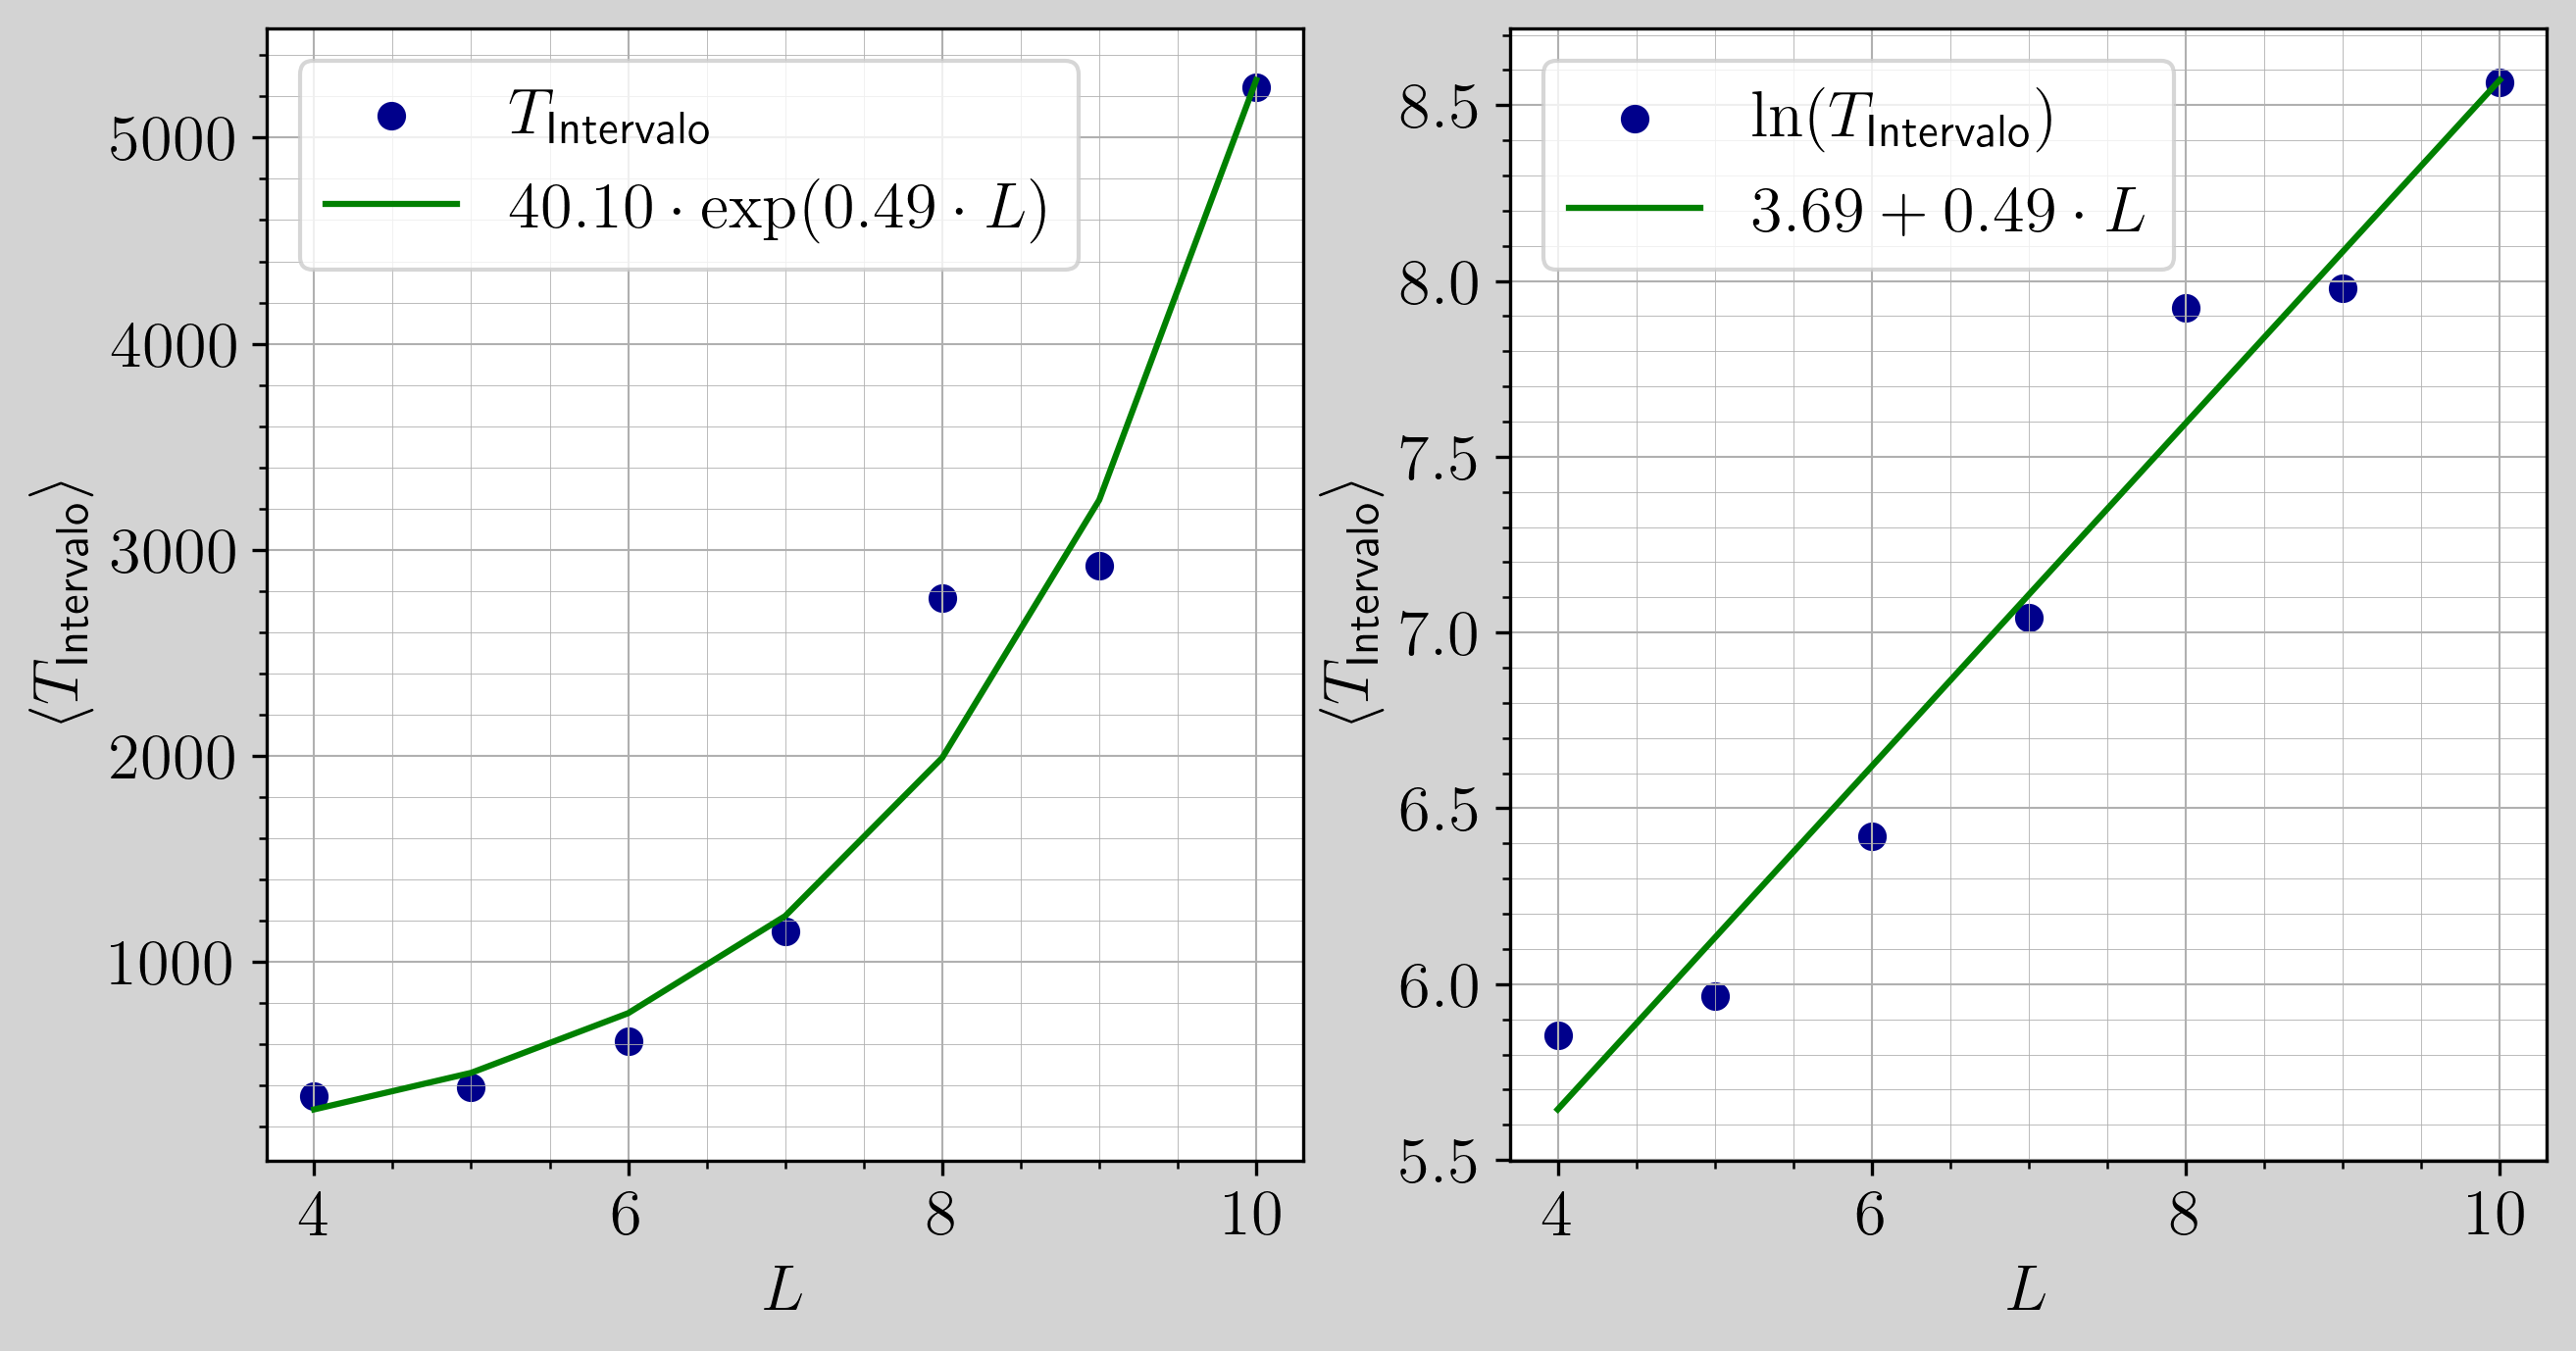
\includegraphics[width=\linewidth]{graficos/tarefa-4/graf-tarefa-D.png}
    \caption{Gráfico do crescimento do intervalo $\langle T_\text{intervalo} \rangle$ em função de $L$ e ajuste linear.}
    \label{fig:d_graficos}
\end{figure}

Para implementação com número de inversões da ordem de $10^4$ foi obtido o ajuste linear 
$\ln\left(\langle T_{\text{intervalo}}(L)\rangle\right)  \approx 3,67 + 0,49 \cdot L$. 

Essa dependência exponencial para que ocorra quebra da simetria talvez explique o que ocorre na simulação da tarefa B
em que o sistema atinge o equilibrio mas a magnetização tem comportamento não usual. Aumentando o número de passos 
de Monte Carlo naquela simulação pode resolver o aparente problema.
\end{document}